% ------------------------------------------------------------------------------------------------
% Journal of Intelligent Manufacturing
% Ver. 1.1 - Reduce repeated wear-state emphasis
% Ver. 1.3 - 16-Apr: LINE 125 
% ------------------------------------------------------------------------------------------------
% RERVISION NOTES
% Green duplication in Intro and Related work? Make Intro. shorter and without citations?
%
% ------------------------------------------------------------------------------------------------

\PassOptionsToPackage{hypertexnames=false}{hyperref}
\documentclass[sn-basic]{sn-jnl} % Basic Springer Nature Reference Style

%% Standard Packages
\usepackage{caption}
\usepackage{subcaption}
\usepackage{graphicx}%
\usepackage{pgfplots}
\pgfplotsset{compat=1.18}
\usepackage{multirow}%
\usepackage{amsmath,amssymb,amsfonts}%
\usepackage{amsthm}%
\usepackage{mathrsfs}%
\usepackage[title]{appendix}%
\usepackage[table]{xcolor}%
\usepackage{textcomp}%
\usepackage{manyfoot}%
\usepackage{booktabs}%
\usepackage{algorithm}%
\usepackage{algorithmicx}%
\usepackage{algpseudocode}%
\usepackage{listings}%
\usepackage{setspace}
\usepackage{xcolor}
\graphicspath{{figures/}}

% NOTE: Draft-only dark theme (commented for submission-ready PDF)
% \pagecolor[rgb]{0.08,0.08,0.10}
% \color[rgb]{0.90,0.90,0.90}
\onehalfspacing
% \lstset{
%         basicstyle=\ttfamily\footnotesize,
%         columns=fullflexible,
%         breaklines=true,
%         frame=single,
%         xleftmargin=0.5em,
%         xrightmargin=0.5em,
%         aboveskip=0.8em,
%         belowskip=0.8em
% }

\begin{document}

\title[Lightweight RL for Edge PdM]{Lightweight Reinforcement Learning for Edge Predictive Maintenance: An Empirical Study of REINFORCE with Attention Mechanisms for Milling Tool Replacement (V.1.3)}


\author[1,4]{\fnm{Rajesh} \sur{Siraskar} \sfx{(\href{https://orcid.org/0000-0003-2341-8787}{ORCID: 0000-0003-2341-8787}})}\email{rajesh.siraskar@gmail.com}
\author*[1,2]{\fnm{Satish} \sur{Kumar}}\email{satish.kumar@sitpune.edu.in}
\author[1,2]{\fnm{Shruti} \sur{Patil}}
\author[1]{\fnm{Arunkumar} \sur{Bongale}}
\author[1,2]{\fnm{Ketan} \sur{Kotecha}}
\author[3]{Ambarish Kulkarni}

\affil*[1]{\orgdiv{Symbiosis Institute of Technology}, \orgname{Symbiosis International (Deemed University)}, \orgaddress{\city{Pune}, \postcode{412115}, \state{Maharashtra}, \country{India}}}
\affil[2]{\orgdiv{Symbiosis Centre for Applied Artificial Intelligence}, \orgname{Symbiosis International (Deemed University)}, \orgaddress{\city{Pune}, \postcode{412115}, \state{Maharashtra}, \country{India}}}
\affil[3]{Swinburne University of Technology, Hawthorn VIC 3122, Australia}
\affil[4]{\orgdiv{CTO Office}, \orgname{Birlasoft Ltd.}, \orgaddress{\city{Pune}, \postcode{411057}, \state{Maharashtra}, \country{India}}}

\abstract{Edge-oriented predictive maintenance (PdM) in Industry~4.0 settings requires decision models that operate under constraints on memory, latency, and energy. This paper examines whether the Monte-Carlo policy-gradient algorithm \textsc{REINFORCE} can provide a competitive lightweight reinforcement-learning (RL) approach for milling-tool replacement when combined with attention-based feature extraction.

The study considers the decision of when to replace a milling cutter under asymmetric costs: replacing too late risks quality loss or failure, whereas replacing too early wastes remaining tool life. We compare four RL algorithms (\textsc{A2C}, \textsc{DQN}, \textsc{PPO}, and \textsc{REINFORCE}) and four attention mechanisms (Nadaraya--Watson, temporal, multi-head, and self-attention). Focused on industrial practitioners, we build an AutoRL workflow for standardized training, repeated evaluation, and consolidated reporting.

A Gymnasium-compatible PdM environment is developed with a schema-adaptive observation design built around measurements available during cutting. Experiments on two milling datasets with different sensing modalities---the public IEEE PHM~2010 benchmark and an in-house university dataset---indicate that, under the adopted evaluation protocol, \textsc{REINFORCE} serves as a strong lightweight baseline: it performs more strongly than \textsc{A2C} and \textsc{DQN} while remaining comparable to \textsc{PPO}. Attention mechanisms are also beneficial overall, although the most effective variant depends on the dataset. Taken together, these findings support \textsc{REINFORCE} as a lightweight baseline for edge-oriented PdM.}

\keywords{Predictive maintenance, Industry 4.0, Edge computing, Reinforcement Learning, REINFORCE, Attention mechanisms, Sustainable AI, AutoRL}

\maketitle

\section{Introduction}
\subsection{Background}
Predictive maintenance (PdM) aims to intervene before functional failure while maximizing asset utilization and protecting product quality. In Industry~4.0 deployments, sensorized manufacturing equipment generates rich telemetry streams that enable condition-aware decision support and prescriptive control \cite{Zonta2020, Compare2020}. In practical settings, however, PdM decision support increasingly needs to operate at the \emph{edge} (close to machines) to reduce latency and bandwidth requirements and to improve reliability in the presence of connectivity or cloud-service disruptions.

Edge deployment introduces hard constraints on compute cycles, memory footprint, and energy consumption. These constraints motivate \emph{lightweight} learning methods and also support the ``Green AI'' initiative. During the training phase, when many candidate agents are explored in sweep-based experimentation, the incremental cost per run becomes operationally and environmentally relevant \cite{Schwartz2020, Strubell2019}. During inference, lighter models with smaller serialized sizes are better aligned with edge-compute requirements.

\subsection{Problem statement}
This paper studies a prescriptive PdM decision: what is the optimum time to replace a milling cutting tool? The decision is cost-asymmetric: late replacement risks defective parts or failure, while early replacement disrupts production and reduces usable tool life. In practical milling, direct wear inspection typically requires interrupting machining and removing the tool from the spindle, so online decisions must be made from in-process machine measurements rather than from direct wear measurements. Reinforcement learning is a natural fit because the agent must trade off utilization against risk over time under edge-oriented resource limits.

The core research question we try to address is: \emph{Can a computationally light policy-gradient algorithm such as \textsc{REINFORCE} remain competitive with more advanced deep RL methods such as \textsc{DQN}, \textsc{A2C}, and \textsc{PPO} for milling PdM when paired with attention-based feature extraction?}

\subsection{Contributions}

This study builds on evidence that na\"{i}ve \textsc{REINFORCE} can perform strongly for PdM in untuned regimes \cite{Siraskar2025} and on prior PdM work using a Nadaraya--Watson estimator as a lightweight attention mechanism under edge constraints \cite{Siraskar2024}. AutoRL is used here as an implementation framework that standardizes training and evaluation across a grid of algorithmic and hyperparameter choices, producing comparable artefacts (dashboards, heatmaps, and hypothesis-test summaries) for model selection when exhaustive manual tuning is impractical \cite{Schwartz2020, Strubell2019, Faust2019, Mussi2022}.

\textbf{Research objectives and hypotheses.}
The study addresses the following research objectives: (1) compare RL algorithms suitable for edge-oriented PdM, (2) evaluate whether \textsc{REINFORCE} is a competitive lightweight baseline, (3) assess attention mechanisms as a form of inductive bias that can improve lightweight RL when decisions are made from measurements available during cutting, (4) design a Gymnasium-compatible RL environment that operates across differing sensor schemas, and (5) provide, for the convenience of industrial practitioners, an AutoRL system for experimentation and training.

We test three hypotheses:
\begin{itemize}
        \item \textbf{H1 (primary):} A computationally light \textsc{REINFORCE} agent is competitive with \textsc{A2C}, \textsc{DQN}, and \textsc{PPO} on the studied PdM task.
        \item \textbf{H2:} The same environment design and reward logic can be applied effectively across two different milling-machine schemas (SIT and IEEE).
        \item \textbf{H3:} Attention mechanisms can improve \textsc{REINFORCE} performance.
\end{itemize}

\textbf{Contributions.}
This paper contributes:
\begin{itemize}
        \item \textbf{Lightweight RL evidence for edge PdM:} an empirical comparison showing when \textsc{REINFORCE} is competitive against \textsc{A2C}, \textsc{DQN}, and \textsc{PPO} on a milling tool-replacement PdM task driven by online machine observations.
        \item \textbf{Attention mechanisms as inductive bias for lightweight RL:} Nadaraya--Watson, temporal attention, multi-head attention, and self-attention implemented as feature extractors for RL policies.
        \item \textbf{A schema-adaptive Gymnasium environment:} a milling-tool PdM environment built around online process measurements across different sensor schemas \cite{Foundation2023}.
        \item \textbf{Practitioner convenience mechanism (AutoRL):} batch training and multi-round evaluation with checkpointed recovery and standardized reporting to reduce the burden of manual tuning and ad-hoc experimentation.
\end{itemize}

\section{Related Work}
\subsection{PdM, Industry~4.0, and edge constraints}
PdM is commonly positioned as an Industry~4.0 centerpiece because it links sensing, connectivity, analytics, and operational decision-making in cyber-physical production systems \cite{Compare2020, Zonta2020}. Prescriptive maintenance architectures further enhance this role by embedding \emph{prescriptive} decision-making, such as suggesting the \emph{action} to take directly into cyber-physical workflows \cite{Ansari2019}. Edge deployment strengthens the PdM case by enabling low-latency, resilient operation near equipment, but it also introduces feasibility constraints: memory, compute, latency, and system-integration overhead can limit the practical adoption of complex ML/RL pipelines \cite{Njor2024, Pandey2023}. These constraints relate to sustainability and ``Green AI'' concerns: when many candidate agents are trained during AutoRL exploration, the incremental cost per training run becomes operationally and environmentally relevant \cite{Schwartz2020, Strubell2019}.

\subsection{RL for predictive maintenance}
RL has been surveyed extensively in PdM, with evidence that a wide range of formulations have been explored across maintenance scheduling, inspection, and resource-constrained decision problems \cite{Siraskar2023, Ogunfowora2023, Zhang2024}. A consistent theme across these surveys is that the ``right'' RL complexity level depends on (i) the structure of the decision problem (action-space size, time horizon and the rewards occurence frequency within that) and (ii) deployment requirements (compute, memory, latency).

The literature also suggests a useful two-stream picture. Many PdM and condition-based maintenance studies learn effective policies using non-deep or otherwise lightweight RL, especially when state representations are structured and action spaces are modest \cite{Adsule2020, Yousefi2020, Rasay2024, Dadash2024}. Deep RL (e.g., DQN/PPO-style methods) becomes more prominent as environments become richer and harder: higher-dimensional sensing, long-horizon tradeoffs, multi-component scheduling, or coupled resource constraints \cite{Liu2020, Chen2023, Lee2022, Ong2022-02}.

\subsection{Lightweight RL for edge PdM}
The literature does not establish that REINFORCE is universally better than advanced deep RL, but it does indicate that lightweight methods are often a sound engineering choice when the PdM task is structured and edge constraints are first-order requirements \cite{Compare2020, Njor2024, Pandey2023}. In embedded RL more broadly, deep RL frequently requires additional techniques such as transfer learning, pruning, compression, or distillation, to fit constrained edge devices \cite{Jang2020, Szydlo2022, Xu2022}.

%% $$$ REFINE
Sustainability motivation: While maintenance optimization contributes to energy and emissions objectives in industrial systems, the PdM literature rarely reports \emph{algorithm-level} energy drawn or carbon footprints for employing RL methods, \cite{Banyai2021, Banyai2022, JasiulewiczKaczmarek2024}. In the empirical study \cite{Siraskar2025}, conducted across 15 environment variants and 10 rounds of training and testing, REINFORCE achieved the highest reported tool-replacement precision at 0.687, exceeding the next-best method by 0.215 in absolute terms; the same study reports that REINFORCE also led the other algorithms on recall, F1, and $F_{\beta=0.5}$. The reported model sizes were small: 56.4~KB for DQN, 89.8~KB for A2C, 121.5~KB for REINFORCE, and 135.5~KB for PPO \cite{Siraskar2025}.

``Green AI'' claims in this paper is provided as \emph{downstream} implications of reduced computational demand and not as scientifically measured environmental outcomes. 

A second quantitative anchor comes from richer IIoT maintenance decision problems where heavier DRL can earn its place. Ong et al.~report that a PPO--LSTM based PdM framework outperformed comparable DRL methods by 53\% and human participants by 65\% in a maintenance resource-management simulator \cite{Ong2022-01}. In a follow-on study, the same line of work introduced transfer learning with demonstrations to reduce DRL training wall time by 58\% \cite{Ong2022-02}.

A third quantitative anchor comes from edge deployment studies that make the memory bottleneck concrete. Pandey et al.~show that in a PdM edge-deployment study, pruning could reduce model sizes dramatically while keeping the average accuracy drop within about 3 percentage points \cite{Pandey2023}. For example, with STFT features, AlexNet was reduced from 28,534,479 to 75,627 parameters (accuracy 98.37\% to 97.65\%), while LeNet fell from 76,695 to 1,967 parameters (accuracy 98.07\% to 97.13\%) \cite{Pandey2023}. With CWT features, AlexNet fell from 28,534,479 to 656,620 parameters \cite{Pandey2023}. The implication is not that deep models are unusable, but that their deployment often depends on pruning, quantization, distillation, or related compression steps before edge feasibility can be discussed \cite{Pandey2023, Jang2020, Xu2022}.

\begin{table}[t]
        \centering
        \small
        \setlength{\tabcolsep}{4pt}
        \begin{tabular}{p{0.24\textwidth} p{0.42\textwidth} p{0.30\textwidth}}
                \toprule
                Evidence strand & Quantitative anchor & Reviewer-safe reading \\
                \midrule
                Direct REINFORCE evidence in PdM & REINFORCE leads tool-replacement precision at 0.687 across 15 variants, and reported model sizes remain small (56.4~KB DQN, 89.8~KB A2C, 121.5~KB REINFORCE, 135.5~KB PPO) \cite{Siraskar2025} & A simple policy-gradient baseline can be competitive in PdM and is not disqualified on footprint grounds \\
                Richer IIoT maintenance decision problems & PPO--LSTM outperforms comparable DRL methods by 53\% and human participants by 65\% in a maintenance resource-management simulator \cite{Ong2022-01} & As the decision problem becomes richer and more coupled, heavier DRL can earn its place \\
                Cost of making DRL practical & Transfer learning with demonstrations cuts DRL training wall time by 58\% \cite{Ong2022-02} & Stronger DRL performance often comes with extra algorithmic machinery and training burden \\
                Edge deployment bottleneck & AlexNet with STFT features shrinks from 28,534,479 to 75,627 parameters with accuracy moving from 98.37\% to 97.65\% after pruning \cite{Pandey2023} & Memory headroom is a hard engineering constraint, not a vague concern \\
                \bottomrule
        \end{tabular}
        \caption{Quantitative anchors supporting a reviewer-safe positioning of lightweight RL for edge-aware PdM.}
        \label{tab:quantitative_anchors_lightweight_edge}
\end{table}
\section{Background / Preliminary Knowledge}
\subsection{MDP notation and observation model}
We model milling PdM as a sequential decision problem. An episodic Markov Decision Process (MDP) is defined by $(\mathcal{S},\mathcal{A},P,R,\gamma)$, where $\mathcal{S}$ is the state space, $\mathcal{A}$ is the action space, $P(s'\mid s,a)$ is the transition kernel, $R(s,a)$ is the reward function, and $\gamma\in(0,1]$ is the discount factor.

In the studied PdM setting, the policy receives a sensor vector $\mathbf{x}_t\in\mathbb{R}^d$ derived from multiple channels rather than a fully instrumented machine-condition state. Direct wear inspection is not modeled as an online input because obtaining it during milling would require interrupting the operation and removing the tool. We therefore formulate the controller around the information that is actually available during cutting and treat representation learning from these process measurements as a first-order factor in policy performance.
\label{sec:obs_model}
\subsection{RL algorithms compared}
\label{sec:algos}
We compare four algorithms: DQN (value-based), A2C (actor--critic), PPO (policy optimization), and REINFORCE (Monte-Carlo policy gradient).

\subsubsection{REINFORCE (Monte-Carlo policy gradient)}
REINFORCE directly estimates the policy gradient using Monte-Carlo returns \cite{Williams1992}:
\begin{equation}
\nabla_\theta J(\theta) = \mathbb{E}\left[\sum_{t=0}^{T} \nabla_\theta \log \pi_\theta(a_t\mid s_t)\,\big(G_t-b(s_t)\big)\right].
\end{equation}

\subsubsection{A2C (advantage actor--critic)}
Actor--critic methods use a learned value baseline $V_\phi(s_t)$ to reduce variance. With advantage estimate $\hat{A}_t=G_t-V_\phi(s_t)$, the policy gradient takes the form
\begin{equation}
\nabla_\theta J(\theta) \approx \mathbb{E}\big[\nabla_\theta\log\pi_\theta(a_t\mid s_t)\,\hat{A}_t\big].
\end{equation}
The critic is trained by minimizing a regression loss such as
\begin{equation}
\mathcal{L}_V(\phi)=\mathbb{E}\big[(G_t - V_\phi(s_t))^2\big].
\end{equation}

\subsubsection{PPO (clipped policy optimization)}
PPO constrains policy updates using a clipped surrogate objective \cite{Schulman2017}. Define the probability ratio
\begin{equation}
 r_t(\theta)=\frac{\pi_\theta(a_t\mid s_t)}{\pi_{\theta_{\mathrm{old}}}(a_t\mid s_t)}.
\end{equation}
With advantage $\hat{A}_t$, the clipped objective is
\begin{equation}
\mathcal{L}^{\mathrm{CLIP}}(\theta)=\mathbb{E}\left[\min\Big(r_t(\theta)\hat{A}_t,\;\mathrm{clip}(r_t(\theta),1-\epsilon,1+\epsilon)\hat{A}_t\Big)\right].
\end{equation}
In typical implementations, the optimized objective also includes a value-function penalty and an entropy bonus:
\begin{equation}
\mathcal{J}(\theta,\phi)=\mathcal{L}^{\mathrm{CLIP}}(\theta) - c_1\,\mathcal{L}_V(\phi) + c_2\,H(\pi_\theta).
\end{equation}

\subsubsection{DQN (deep Q-learning)}
DQN learns an action-value function $Q_\theta(s,a)$ and minimizes a temporal-difference error with a target network \cite{Mnih2015}:
\begin{equation}
\mathcal{L}(\theta)=\mathbb{E}\left[\left(r_t + \gamma\max_{a'}Q_{\bar\theta}(s_{t+1},a') - Q_\theta(s_t,a_t)\right)^2\right].
\end{equation}
Experience replay and target-network updates stabilize learning, but performance can still degrade when the observed sensor vector does not fully summarize the underlying degradation state without explicit memory.

\subsubsection{Why REINFORCE can be edge-suited}
When deployment constraints are first-order requirements, algorithmic simplicity can translate to smaller policies and lower training/inference overhead. In sweep-based experimentation (including AutoRL-style grids), simpler learners can also reduce total compute when many configurations must be compared. This does not guarantee superior reward, but it shifts the burden of proof: if a lightweight method is statistically competitive on PdM metrics, it may be preferable for edge-first deployments \cite{Schwartz2020, Njor2024}.

\section{Methodology and Experimental Setup}
\label{sec:method}
\subsection{Problem formulation: asymmetric costs and decision rationale}
\label{sec:problem}
PdM decisions are inherently asymmetric. A late replacement can cause defective parts, scrap, or catastrophic failure, while an early replacement wastes remaining tool life.

\begin{table}[t]
        \centering
        \caption{Conceptual cost-aware interpretation of PdM decisions (qualitative), aligned with the reward shaping in Section~\ref{sec:reward}.}
        \label{tab:cost_view}
        \begin{tabular}{p{0.18\linewidth} p{0.32\linewidth} p{0.42\linewidth}}
                \toprule
                \textbf{Case} & \textbf{Condition} & \textbf{PdM interpretation}\\
                \midrule
                Timely replace & $a_t=0$ near $w\approx\tau$ & Desired: high utilization and low violation risk.\\
                Early replace & $a_t=0$ when $w\ll\tau$ & Safe but wasteful: reduces risk while discarding useful life.\\
                Late action / violation & $a_t=1$ while $w>\tau$ & Worst case: elevated risk of quality loss or failure; strongly penalized.\\
                Continue safely & $a_t=1$ with $w<\tau$ & Encouraged: extracts remaining useful life when safe.\\
                \bottomrule
        \end{tabular}
\end{table}

\subsection{Algorithm description}
\label{sec:algo_desc}
\subsubsection{AutoRL as a practitioner convenience: standardized sweeps and reporting}
\label{sec:autorl}
The AutoRL pipeline is implemented as a CLI batch runner (\texttt{code/batch\_train.py}) that supports training, evaluation, and reporting across a grid of algorithms, hyperparameters, and attention mechanisms. The pipeline is designed to be practitioner-friendly in two ways:
\begin{itemize}
        \item \textbf{Automation:} algorithm and attention choices are enumerated automatically; evaluation is repeated for multiple rounds.
        \item \textbf{Reliability:} long-running sweeps use a lightweight SQLite checkpoint queue to recover from failures without manual intervention.
\end{itemize}
For this study, multi-round evaluation uses 20 rounds (\texttt{EVAL\_ROUNDS=20}) to support confidence intervals and statistical tests.

\subsubsection{Training procedure and policy architecture}
All agents are trained using Stable-Baselines3 with an \texttt{MlpPolicy} and a Gymnasium-compatible environment wrapper. Each training run uses a fixed number of episodes (\texttt{EPISODES=100}) with early stopping triggered by an episode-count callback, and learning rate $\eta$ and discount factor $\gamma$ are swept as part of the AutoRL grid.

Attention mechanisms are implemented as custom feature extractors $\phi(\mathbf{x}_t)$ that map the raw sensor observation $\mathbf{x}_t$ into a 64-dimensional embedding (\texttt{features\_dim=64}). The resulting embedding is then consumed by the default multilayer-perceptron policy/value networks provided by Stable-Baselines3.

\subsubsection{Attention mechanisms as lightweight feature extractors}
\label{sec:attention}
Because the policy acts on sensor vectors rather than on a fully instrumented machine state (Section~\ref{sec:obs_model}), the core challenge becomes representation learning from multivariate observations. Attention is a representation-learning prior that biases the policy toward informative sensor patterns and feature interactions. We implement attention mechanisms as feature extractors $\phi_\theta(\mathbf{x}_t)$ that map a raw sensor vector into a compact embedding used by the RL policy.

\textbf{General attention concept.}
Given values $V=\{\mathbf{v}_1,\ldots,\mathbf{v}_n\}$ and a query $\mathbf{q}$, attention forms a convex combination
\begin{equation}
\mathrm{Attention}(\mathbf{q},V)=\sum_{i=1}^{n}\alpha_i\,\mathbf{v}_i,\qquad \sum_i\alpha_i=1,\;\alpha_i\ge 0,
\end{equation}
with weights computed by a softmax over a compatibility score $s(\mathbf{q},\mathbf{v}_i)$:
\begin{equation}
\alpha_i = \frac{\exp(s(\mathbf{q},\mathbf{v}_i))}{\sum_{j=1}^n\exp(s(\mathbf{q},\mathbf{v}_j))}.
\end{equation}

\textbf{Note on terminology.}
We use ``attention'' as a unifying label for feature extractors that implement (i) learned reweighting/gating and (ii) structured fusion of sensor features and (optionally) time context. In this sense, attention provides a structured way to weight informative features and feature interactions, which can improve learning in this measurement-constrained setting.

\paragraph{Nadaraya--Watson attention (NW)}
NW attention can be interpreted as kernel-regression-based soft retrieval from learnable prototypes. This mechanism is computationally light and aligns with prior PdM attention work motivated by edge constraints \cite{Siraskar2024}.

A standard Gaussian-kernel form is
\begin{equation}
\alpha_i = \frac{\exp\left(-\tfrac{\lVert \mathbf{k}_i-\mathbf{q}\rVert^2}{2\sigma^2}\right)}{\sum_j \exp\left(-\tfrac{\lVert \mathbf{k}_j-\mathbf{q}\rVert^2}{2\sigma^2}\right)},
\qquad \mathbf{z}=\sum_i\alpha_i\,\mathbf{v}_i.
\end{equation}

\begin{algorithm}[t]
\caption{NW attention feature extractor (forward pass)}
\label{alg:nw_forward}
\begin{algorithmic}[1]
\Require observation vector $\mathbf{x}$; learnable prototype keys $\{\mathbf{k}_i\}$ and values $\{\mathbf{v}_i\}$; query network $f_\theta$; parameter $\log\beta$
\Ensure context feature $\mathbf{z}$
\State $\mathbf{q} \gets f_\theta(\mathbf{x})$ \Comment{query}
\For{$i \gets 1$ to $N$}
        \State $d_i \gets \lVert \mathbf{q}-\mathbf{k}_i\rVert^2$
\EndFor
\State $\beta \gets \exp(\log\beta)$ \Comment{enforce $\beta>0$}
\State $\alpha \gets \mathrm{softmax}(-\beta\,\mathbf{d})$ \Comment{normalize over prototypes}
\State $\mathbf{z} \gets \sum_{i=1}^{N} \alpha_i\,\mathbf{v}_i$
\State \Return $\mathbf{z}$
\end{algorithmic}
\end{algorithm}

\paragraph{Temporal attention (TP)}
Temporal attention injects an explicit stage-of-life signal using sinusoidal positional encodings and a learnable temporal embedding \cite{Vaswani2017}.

\begin{algorithm}[t]
\caption{Temporal attention feature extractor (forward pass)}
\label{alg:tp_forward}
\begin{algorithmic}[1]
\Require observation vector $\mathbf{x}$; spatial attention network $g_\theta$; positional encodings $\mathrm{PE}[\cdot]$; temporal embedding $\mathbf{e}$; timestep counter $t$; fusion network $h_\theta$
\Ensure feature embedding $\mathbf{z}$
\State $\mathbf{w} \gets g_\theta(\mathbf{x})$ \Comment{per-channel spatial weights}
\State $\tilde{\mathbf{x}} \gets \mathbf{x} \odot \mathbf{w}$
\State $\mathbf{p} \gets \mathrm{PE}[t \bmod T_{\max}] + \mathbf{e}$
\State $\mathbf{z} \gets h_\theta(\mathrm{concat}(\tilde{\mathbf{x}},\mathbf{p}))$
\State $t \gets t+1$
\State \Return $\mathbf{z}$
\end{algorithmic}
\end{algorithm}

\paragraph{Multi-head attention (MH)}
Multi-head attention uses multiple attention heads to represent different subspaces of sensor relationships \cite{Vaswani2017}.

In standard form,
\begin{align}
\mathrm{head}_h &= \mathrm{Attention}(QW_h^Q,\,KW_h^K,\,VW_h^V),\\
\mathrm{MultiHead}(Q,K,V) &= \mathrm{Concat}(\mathrm{head}_1,\ldots,\mathrm{head}_H)\,W^O.
\end{align}

\begin{algorithm}[t]
\caption{Multi-head attention feature extractor (forward pass; head-gating over $H$ heads)}
\label{alg:mh_forward}
\begin{algorithmic}[1]
\Require observation vector $\mathbf{x}$; projections $W^Q,W^K,W^V$; output projection $W^O$; number of heads $H$; per-head dimension $d$; scale factor $c$
\Ensure feature embedding $\mathbf{z}$
\State $Q \gets (\mathbf{x}W^Q) \rightarrow \text{reshape}(H, d)$
\State $K \gets (\mathbf{x}W^K) \rightarrow \text{reshape}(H, d)$
\State $V \gets (\mathbf{x}W^V) \rightarrow \text{reshape}(H, d)$
\For{$h \gets 1$ to $H$}
        \State $s_h \gets c\,\langle Q_h, K_h\rangle$
\EndFor
\State $\alpha \gets \mathrm{softmax}(\mathbf{s})$ \Comment{normalize over heads}
\For{$h \gets 1$ to $H$}
        \State $\tilde{V}_h \gets \alpha_h\,V_h$
\EndFor
\State $\mathbf{z} \gets (\mathrm{concat}(\tilde{V}_1,\ldots,\tilde{V}_H))W^O$
\State \Return $\mathbf{z}$
\end{algorithmic}
\end{algorithm}

\paragraph{Self-attention (SA)}
Self-attention projects the observation into a feature space and uses a compact Transformer-style block with residual connections and layer normalization.

In standard token-wise form,
\begin{equation}
\mathrm{SelfAttn}(X)=\mathrm{softmax}\left(\frac{XW_Q(XW_K)^\top}{\sqrt{d}}\right)XW_V.
\end{equation}

In this codebase, the softmax normalization is across the \emph{batch} dimension; this can act as a stabilization/gating mechanism, though it differs from token-wise self-attention.

\begin{algorithm}[t]
\caption{Self-attention feature extractor (forward pass; batch-normalized gating)}
\label{alg:sa_forward}
\begin{algorithmic}[1]
\Require mini-batch $\{\mathbf{x}_i\}_{i=1}^{B}$; projections $W^{\mathrm{in}},W^Q,W^K,W^V$; scale factor $c$; FFN; layer norms $\mathrm{LN}_1,\mathrm{LN}_2$
\Ensure output features $\{\mathbf{y}_i\}_{i=1}^{B}$
\For{$i \gets 1$ to $B$}
        \State $\mathbf{h}_i \gets \mathbf{x}_i W^{\mathrm{in}}$
        \State $\mathbf{q}_i \gets \mathbf{h}_i W^Q$; $\mathbf{k}_i \gets \mathbf{h}_i W^K$; $\mathbf{v}_i \gets \mathbf{h}_i W^V$
        \State $s_i \gets c\,\langle \mathbf{q}_i,\mathbf{k}_i\rangle$ \Comment{scalar compatibility score}
\EndFor
\State $\alpha \gets \mathrm{softmax}(\mathbf{s})$ \Comment{normalize across batch index $i$}
\For{$i \gets 1$ to $B$}
        \State $\tilde{\mathbf{v}}_i \gets \alpha_i\,\mathbf{v}_i$
        \State $\mathbf{u}_i \gets \mathrm{LN}_1(\mathbf{h}_i + \tilde{\mathbf{v}}_i)$
        \State $\mathbf{y}_i \gets \mathrm{LN}_2(\mathbf{u}_i + \mathrm{FFN}(\mathbf{u}_i))$
\EndFor
\State \Return $\{\mathbf{y}_i\}_{i=1}^{B}$
\end{algorithmic}
\end{algorithm}

\subsection{Simulation environment: a Gymnasium-compatible milling PdM environment}
\label{sec:env}
\subsubsection{Design goals and schema abstraction}
The environment class \texttt{MT\_Env} (\texttt{code/rl\_pdm.py}) implements the Gymnasium interface \cite{Foundation2023}. A central design goal is schema generality: the same environment logic (episode structure, actions, and reward shaping) should work across different milling-machine sensor schemas.

In the implementation, schema abstraction is achieved by keeping the MDP ``skeleton'' fixed while allowing the observation \emph{feature set} to vary:
\begin{itemize}
        \item \textbf{Fixed across schemas:} the observation is a flat real-valued sensor vector $\mathbf{x}_t\in\mathbb{R}^d$, the action space is binary (replace vs. continue), and the reward/termination logic is driven by an internal wear threshold.
        \item \textbf{Schema-dependent:} the specific sensor columns used to form $\mathbf{x}_t$ (and therefore $d$) are selected based on column names.
\end{itemize}

\textbf{Schema detection.}
The environment detects the schema using available sensor columns (e.g., force and acoustic emission channels for IEEE; vibration, sound, and load-cell channels for SIT). If no known schema signature is found, the implementation falls back to using \emph{all} non-excluded columns as sensor features (excluding \texttt{Time}/\texttt{time}, \texttt{tool\_wear}, and \texttt{ACTION\_CODE}).

\textbf{Practical requirement for new datasets.}
To reuse \texttt{MT\_Env} on a new milling-machine dataset without code changes, the CSV must include a \texttt{tool\_wear} column (used internally for termination and reward) plus one or more numeric sensor columns (used as observations).

\subsubsection{Observation and action spaces}
Only sensor readings available during cutting are included in the observation vector; inspection-based wear values are retained internally for reward and termination. The action space is discrete with two actions: $a=0$ means \emph{replace} (terminates the episode) and $a=1$ means \emph{continue}.

\subsubsection{Reward shaping for asymmetric PdM risk}
\label{sec:reward}
The reward function encourages long tool use without threshold violation, while rewarding timely replacement close to the wear threshold. In the implementation, continuing yields a small positive survival reward $R_1$, violating the wear threshold yields a catastrophic penalty $R_2$, replacement has a small cost $R_3$, and replacement near the threshold earns a strong bonus $R_4$ (with stepped bonuses above 70\%, 80\%, and 90\% wear ratio).

This design reflects a practical PdM asymmetry: a late replacement causing quality loss or failure is substantially worse than an early replacement.


\subsection{Experimental design} \label{sec:experiment} 

We evaluate AutoRL under two datasets with deliberately different sensing modalities: (i) an IEEE benchmark dataset (public PHM 2010 data challenge), and (ii) an in-house SIT dataset collected on a university milling testbed. To align the learning problem with real deployment constraints, the environment observation in \texttt{MT\_Env} contains \emph{only} sensor channels (excluding \texttt{Time}, \texttt{tool\_wear}, and \texttt{ACTION\_CODE}). Sensor units are: force in N, vibration in $g$, AE-RMS (\texttt{acoustic\_emission\_rms}) in V, current in A, sound in V, and load-cell signals in kN (or V after conditioning).

\subsubsection{IEEE benchmark dataset (public PHM 2010)}
The IEEE dataset \cite{PHMdata2010} is from the PHM Society 2010 Data Challenge and targets tool-condition monitoring and remaining useful life estimation for a high-speed CNC milling process. The dataset documentation reports a high-speed CNC platform instrumented with a dynamometer (cutting forces), accelerometers (vibrations), and an acoustic-emission sensor, with signals acquired at 50~kHz per channel. The published cutting conditions include a spindle speed of 10{,}400~rpm, feed rate of 1{,}555~mm/min, radial depth of cut 0.125~mm, and axial depth of cut 0.2~mm.

Following the competition release format, we use the seven sensor columns corresponding to \{\texttt{force\_x}, \texttt{force\_y}, \texttt{force\_z}, \texttt{vibration\_x}, \texttt{vibration\_y}, \texttt{vibration\_z}, \texttt{acoustic\_emission\_rms}\}. In typical descriptions of the apparatus, these channels correspond to cutting-force measurement via a dynamometer, vibration measurement via accelerometers, and acoustic emission summarized as an RMS feature. Five cutter records are used in our experiments (three for training and two for evaluation), matching the standard train/test partitioning.

\subsubsection{SIT in-house dataset (university milling testbed)}
The SIT dataset is collected on a Vertical Milling Centre (VMC) (Jyoti NVU PX10) using an NI data acquisition system and a production-oriented sensor suite. The machine-and-sensor layout (Fig.~\ref{fig:expt-setup-1}) and measurement instruments (DAQ and tool-makers microscope; Fig.~\ref{fig:expt-setup-2}) summarize the in-house setup.

Tool wear is quantified via a tool-makers microscope, with the flank-wear definition illustrated using digital images of a new and a worn insert (Fig.~\ref{fig:tool_images}). Progressive wear snapshots used for annotation/validation are shown in Table~\ref{tab:wearimages}. The experiments span spindle speeds of 800--1{,}200~rpm and feed rates of 20--40~mm/min, with a maximum allowable flank wear of 0.32~mm.

The SIT observation schema includes eight channels aligned with \texttt{MT\_Env}: \{\texttt{Vib\_Spindle}, \texttt{Vib\_Table}, \texttt{Sound\_Spindle}, \texttt{Sound\_table}, \texttt{X\_Load\_Cell}, \texttt{Y\_Load\_Cell}, \texttt{Z\_Load\_Cell}, \texttt{Current}\}, covering vibration, sound, three-axis load, and spindle current signals.

\begin{figure}[h]
                                \centering
                                \includegraphics[width=0.305\linewidth]{Expt_Setup_MillingMachine.png}
                                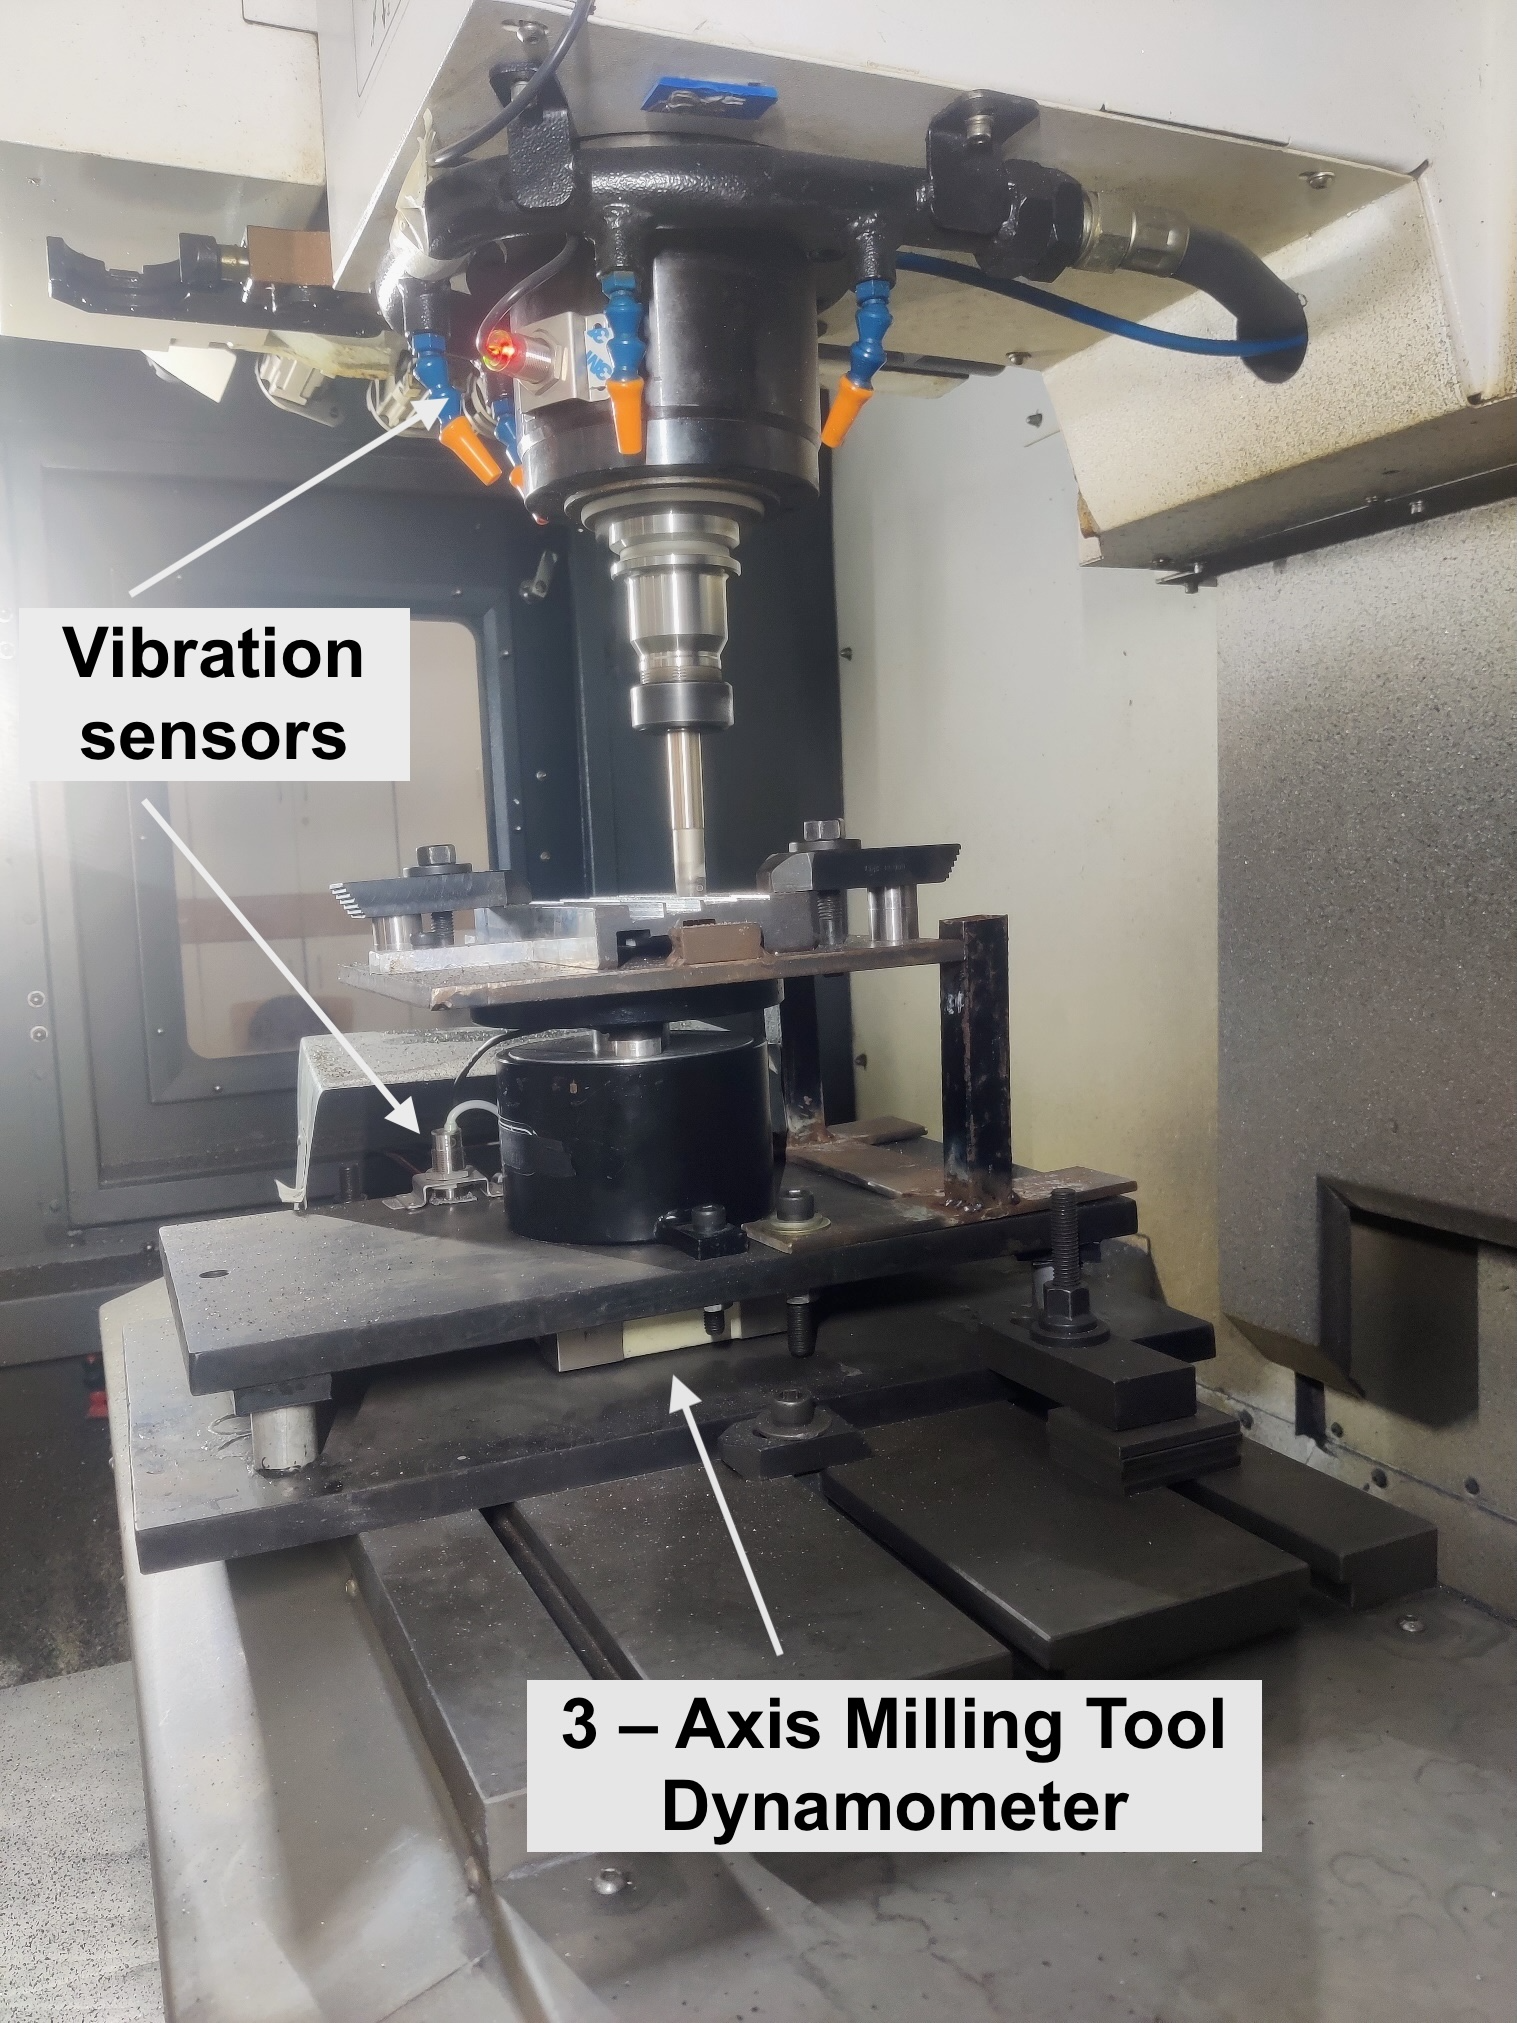
\includegraphics[width=0.45\linewidth]{Expt_Setup_Vibration_and_Dynamometer.png}
                                \caption{Experimental setup - Machine and sensors}
                                \label{fig:expt-setup-1}
\end{figure}

\begin{figure}[h]
                                \centering
                                \includegraphics[width=0.45\textwidth]{Expt_Setup_DACS.png}
                                \includegraphics[width=0.445\textwidth]{Expt_Setup_Microscope.png}
                                \caption{Experimental setups - Measurement instruments}
                                \label{fig:expt-setup-2}
\end{figure}

\begin{table}[h!]
                \centering
                \caption{Progressive tool wear. Images taken using tool-makers microscope}
                \label{tab:wearimages}
                \begin{tabular}{|r|r|c|}
                                \hline
                                Runs & Wear $VB_{max}\mu$m & Tool condition\\
                                \hline
                                 0 &   0.00 & 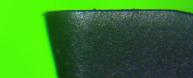
\includegraphics[width=0.3\linewidth]{tw-1.jpg} \\ \hline
                                 5 & 119.71 & 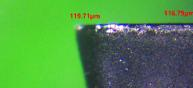
\includegraphics[width=0.3\linewidth]{tw-2.jpg} \\ \hline
                                10 & 170.07 & 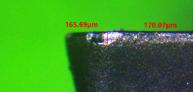
\includegraphics[width=0.3\linewidth]{tw-3.jpg} \\ \hline
                                15 & 212.21 & 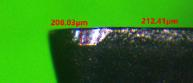
\includegraphics[width=0.3\linewidth]{tw-4.jpg} \\ \hline
                                20 & 236.50 & 
\includegraphics[width=0.3\linewidth]{tw-5.jpg} \\ \hline
                                25 & 254.74 & 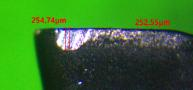
\includegraphics[width=0.3\linewidth]{tw-6.jpg} \\ \hline
                                30 & 280.29 & 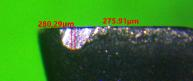
\includegraphics[width=0.3\linewidth]{tw-7.jpg} \\ \hline
                                35 & 303.65 & 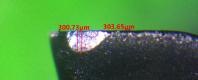
\includegraphics[width=0.3\linewidth]{tw-8.jpg} \\ \hline
                \end{tabular}
\end{table}

\begin{figure}[t]
        \centering
        \begin{subfigure}[t]{0.48\textwidth}
                \centering
                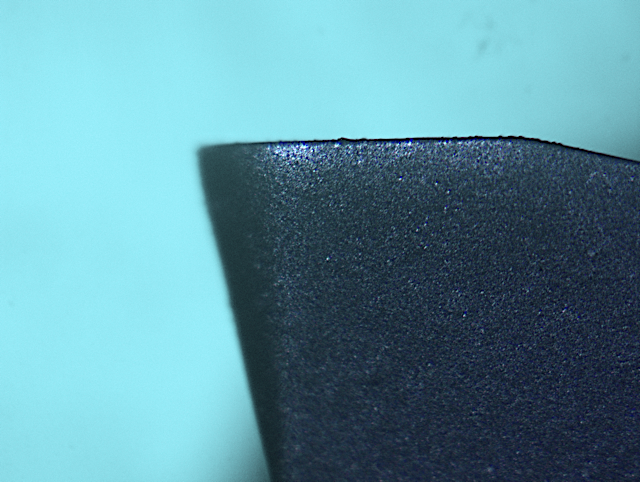
\includegraphics[width=\linewidth]{Tool_New_Insert.png}
                \caption{A tool-insert without wear}
                \label{fig:tool_new}
        \end{subfigure}\hfill
        \begin{subfigure}[t]{0.48\textwidth}
                \centering
                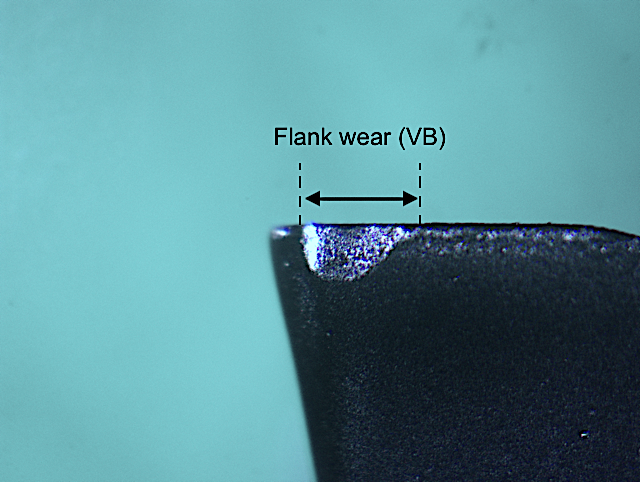
\includegraphics[width=\linewidth]{Tool_Worn Annotated.png}
                \caption{Tool-insert showing wear and how flank-wear (VB) is defined}
                \label{fig:tool_worn}
        \end{subfigure}
        \caption{Milling tool inserts - Digital images using tool-makers microscope}
        \label{fig:tool_images}
\end{figure}

\begin{figure}[t]
        \centering
        \begin{subfigure}[t]{0.48\textwidth}
                \centering
                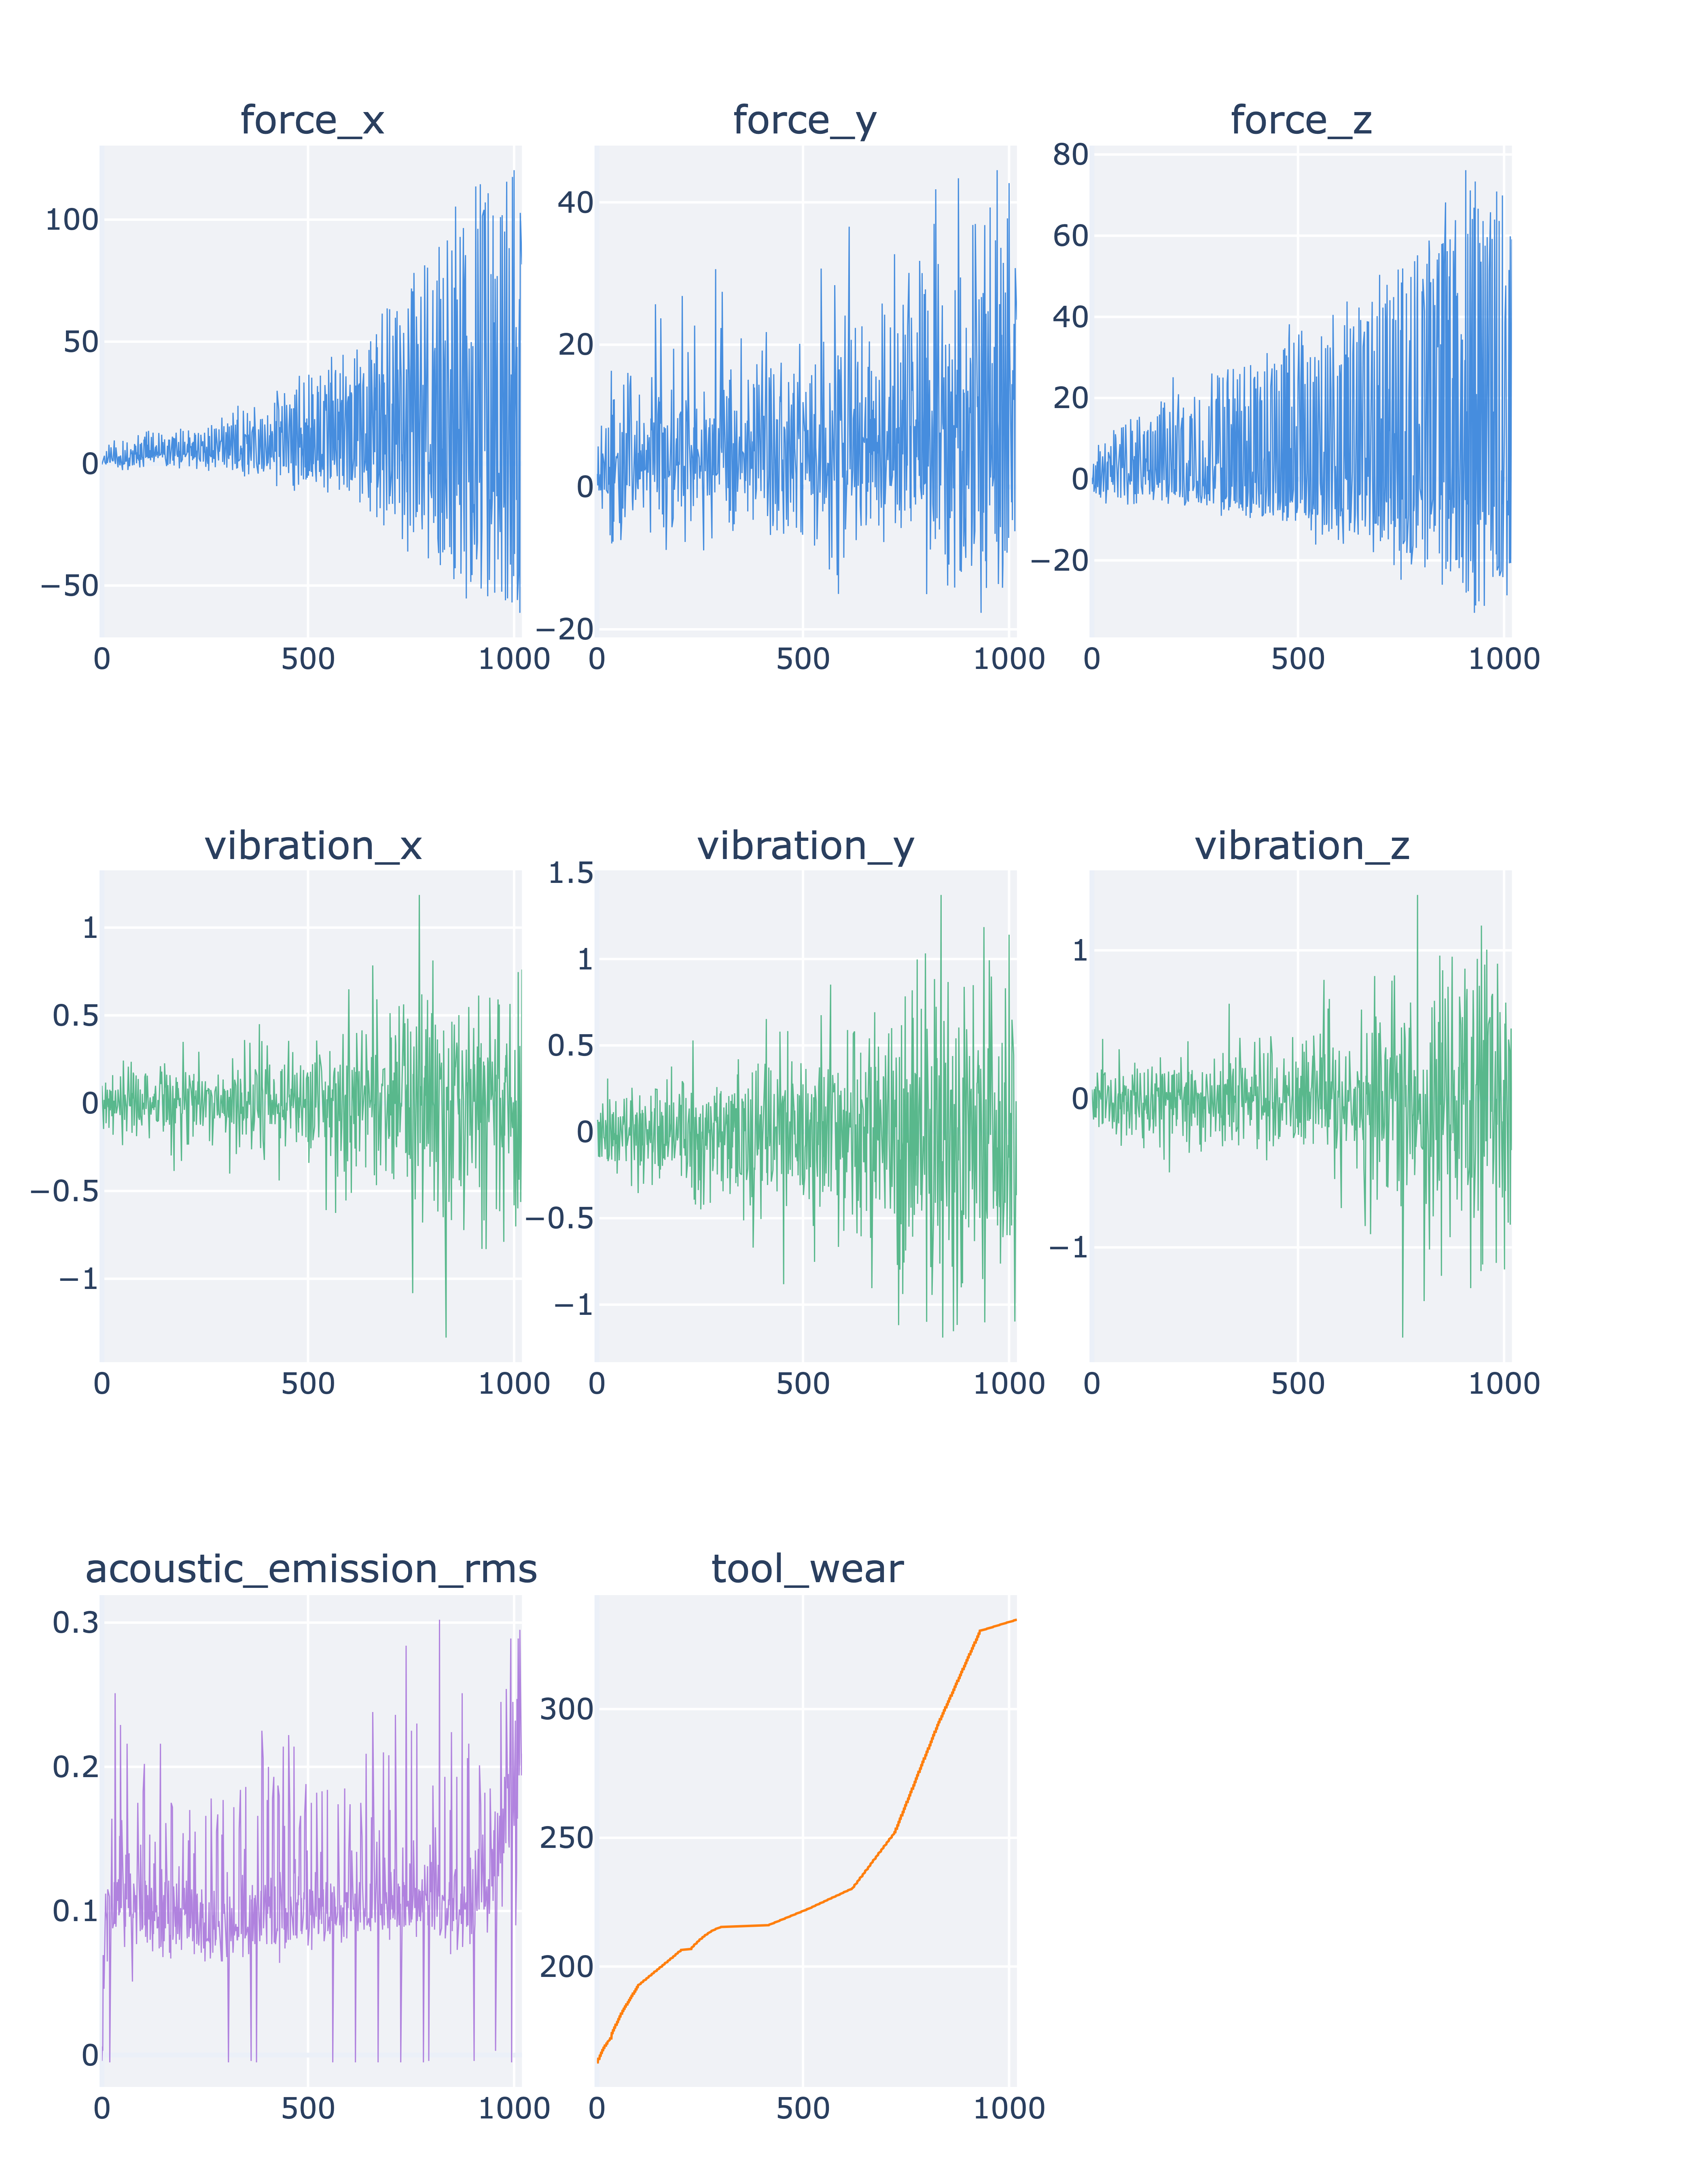
\includegraphics[width=\linewidth]{IEEE_06_SensorPlot.png}
                \caption{IEEE schema features.}
                \label{fig:schema_ieee}
        \end{subfigure}\hfill
        \begin{subfigure}[t]{0.48\textwidth}
                \centering
                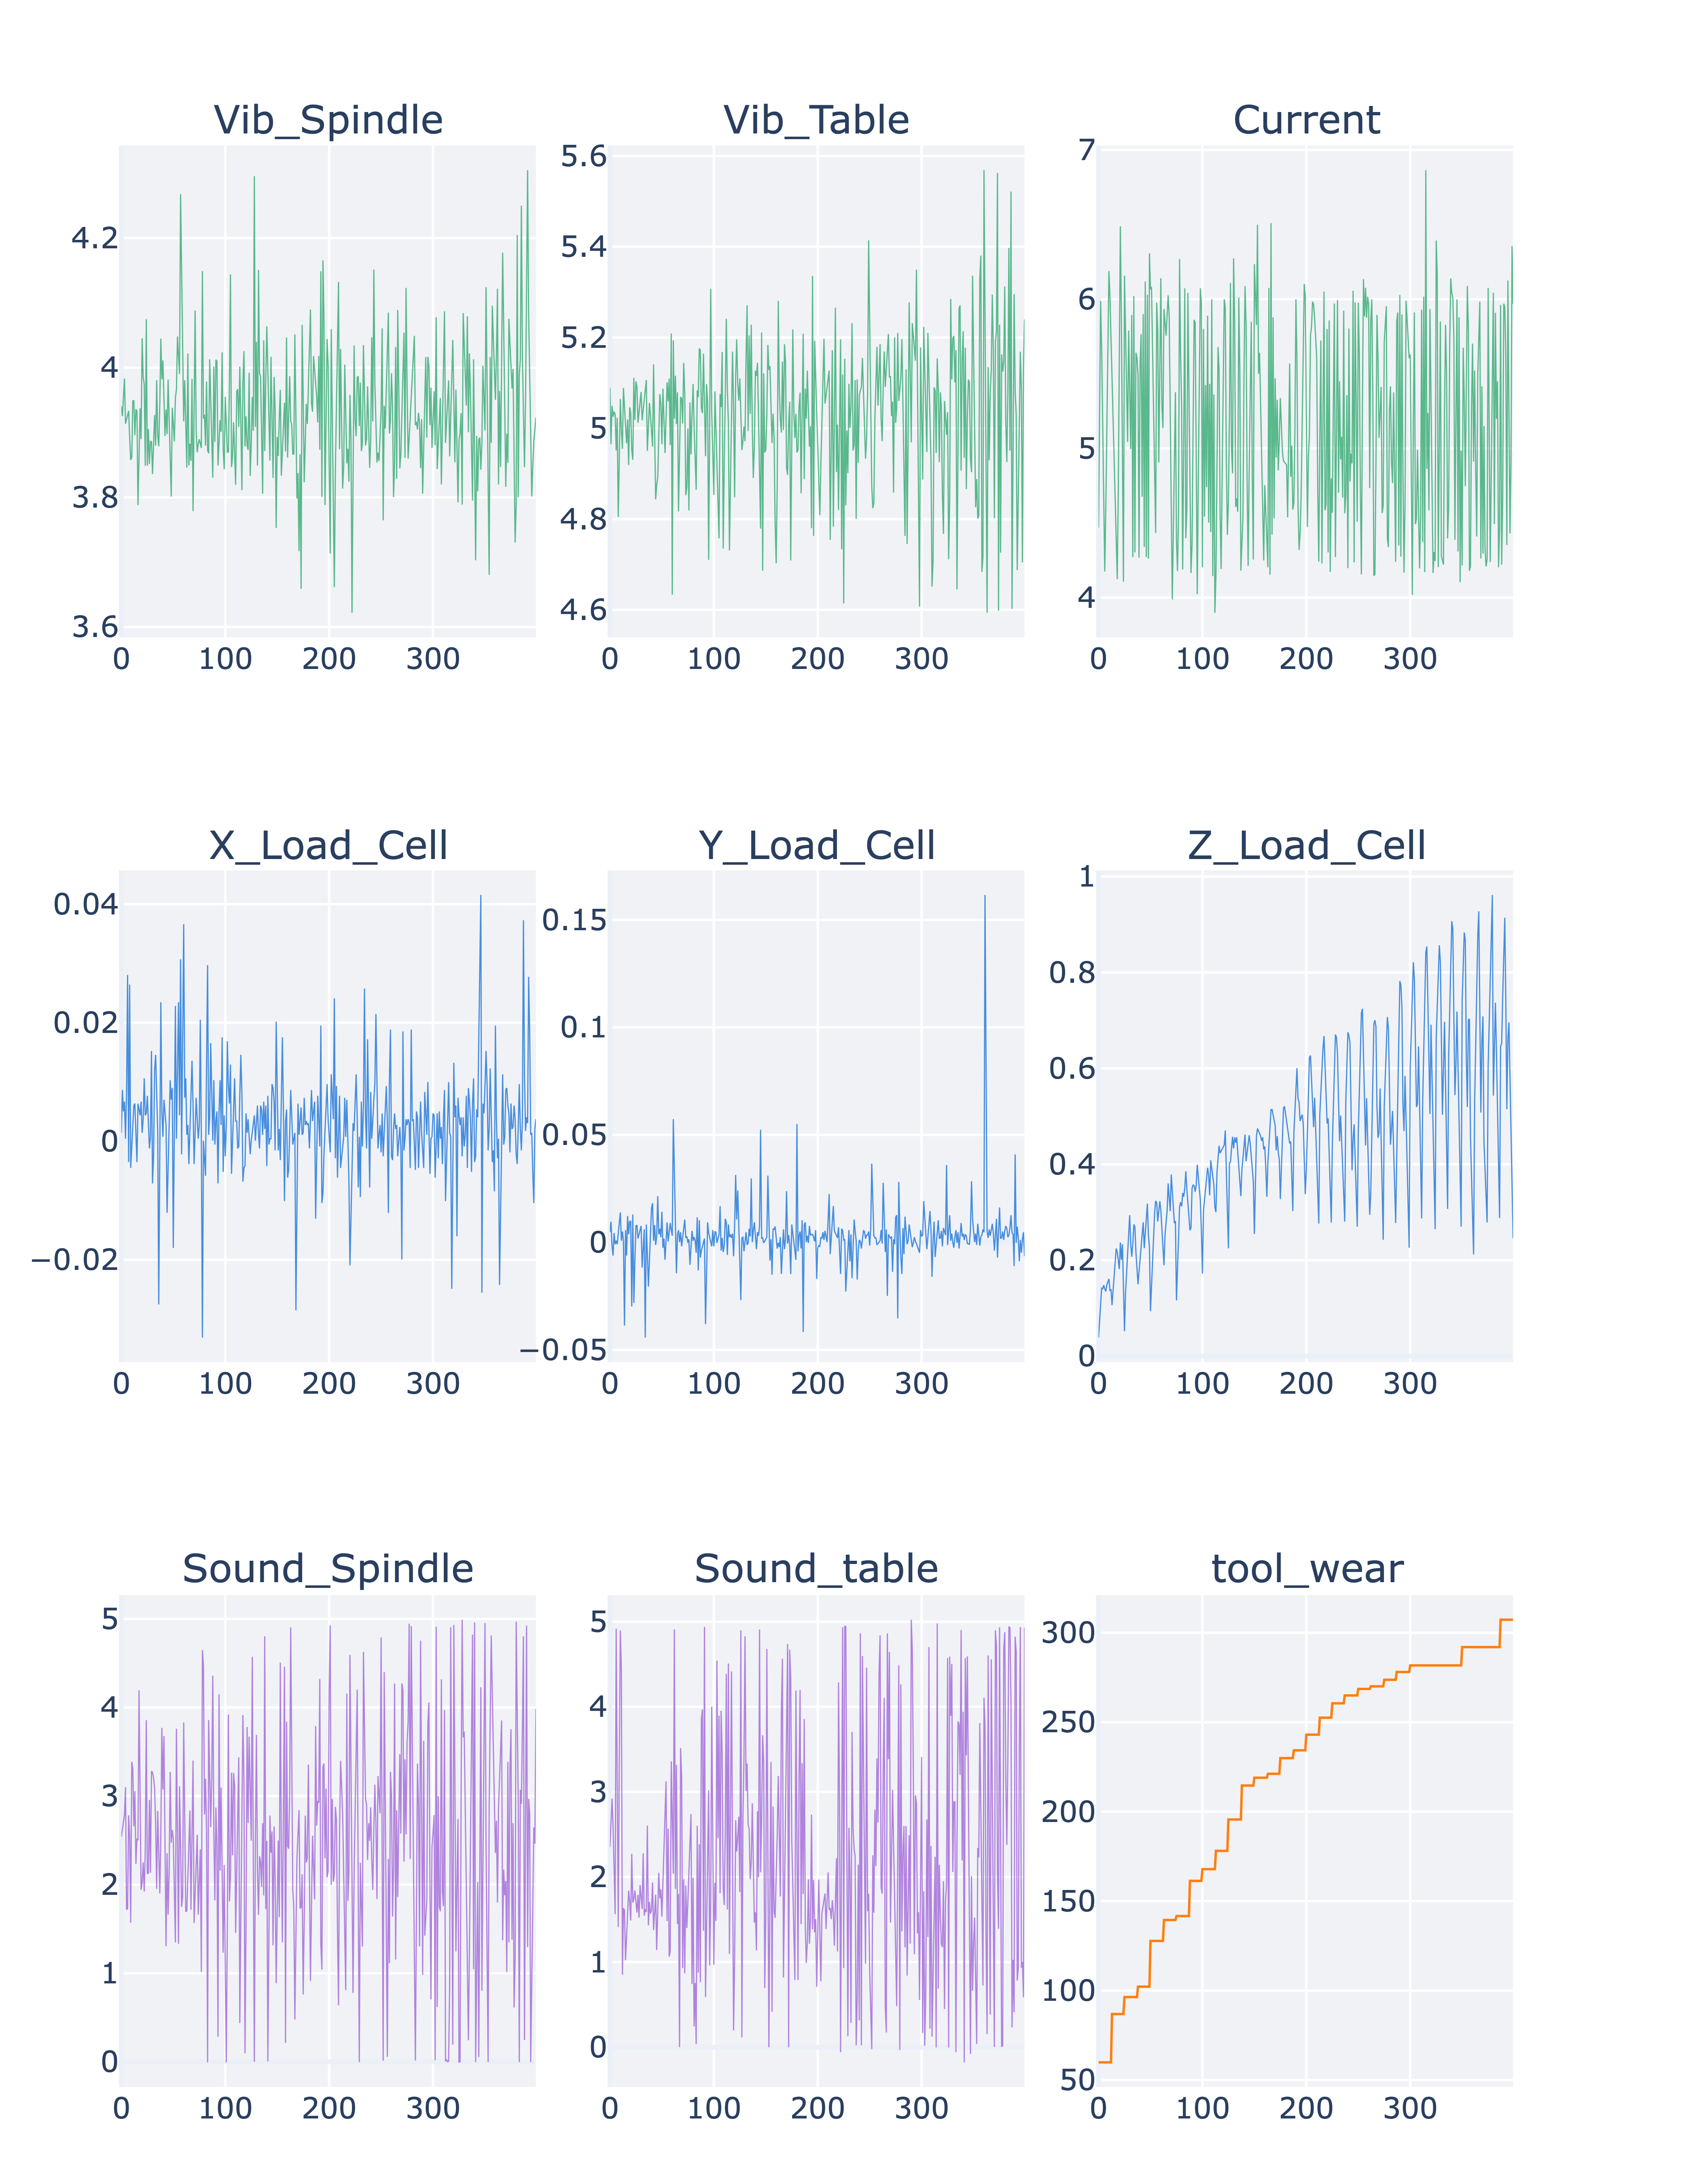
\includegraphics[width=\linewidth]{SIT_20_SensorPlot.png}
                \caption{SIT schema features.}
                \label{fig:schema_sit}
        \end{subfigure}

        \caption{IEEE and SIT schema feature plots: Representational plots depicting differences in sensor features, value ranges, and variations.}
        \label{fig:schema_feature_plots_ieee_sit}
\end{figure}

\textbf{Schema heterogeneity and environment robustness.}
The two schemas differ in both dimensionality (7 vs. 8 channels) and sensing modality (force/vibration/AE vs. vibration/sound/load/current), which produces distinct value ranges and temporal variability patterns (Fig.~\ref{fig:schema_feature_plots_ieee_sit}). This heterogeneity is intentional: \texttt{MT\_Env} selects schema-specific sensor feature sets while keeping the action semantics (replace vs. continue) and wear-threshold termination logic fixed, thereby stress-testing policies built from available machine signals across materially different instrumentation and supporting robustness and generalizability claims.

\subsubsection{Datasets and generalization protocol}
The study uses two sensor schemas: (i) SIT (production-oriented schema with eight sensor channels), and (ii) IEEE (benchmark schema with force, vibration, and acoustic emission channels). Generalization is evaluated via a one-vs-all protocol: agents are trained on training file(s) within a schema and evaluated on remaining unseen files within the same schema.

\subsection{Baselines and metrics}
\label{sec:metrics}
The primary comparison in this paper is among RL agents that consume raw sensor observations directly. We do not include conventional supervised-ML baselines in this version because such pipelines typically require additional target construction, forecasting design choices, or task-specific feature engineering that vary substantially across schemas and practitioner settings. This omission should be treated as a scope choice rather than a claim that conventional ML is unsuitable; adding strong non-RL baselines remains an important extension for future work.

\subsubsection{Evaluation metrics}
We report three metrics used by the AutoRL evaluation: (i) evaluation score, (ii) tool usage (\%), and (iii) a $\lambda$ timing metric.

\subsubsection{Exact evaluation score definition (as implemented)}
The paper-level ``evaluation score'' corresponds to \texttt{calculate\_eval\_score()} in \texttt{code/batch\_train.py}. Let $u\in[0,1]$ be tool usage fraction at first replacement, $v\in\mathbb{N}_0$ be the number of post-threshold timesteps without replacement (threshold violations), and $\lambda=t_{\lambda}-t_{\mathrm{FR}}$ be the signed timing error. The implemented score is
\begin{align}
S_{\text{tool}} &= \mathrm{clip}(u,0,1),\\
S_{\lambda} &= \max\left(0,\,1-\frac{|\lambda|}{c_{\lambda}}\right),\\
S_{\text{viol}} &= \frac{1}{1+v},\\
\mathrm{EvalScore} &= 0.50\,S_{\text{tool}} + 0.30\,S_{\lambda} + 0.20\,S_{\text{viol}}.
\end{align}
Here $c_{\lambda}$ is the normalization constant used by \texttt{calculate\_eval\_score()}, implemented as $c_{\lambda}=\texttt{WEAR\_THRESHOLD}\,(1-\texttt{IAR\_RANGE})$.

\begin{algorithm}[t]
\caption{Evaluation score computation (per evaluation run)}
\label{alg:eval_score}
\begin{algorithmic}[1]
\Require tool usage fraction $u$; timing error $\lambda$; violation count $v$; constants $c_{\lambda}=\texttt{WEAR\_THRESHOLD}\,(1-\texttt{IAR\_RANGE})$
\Ensure scalar score $S\in[0,1]$
\State $S_{\mathrm{tool}} \gets \mathrm{clip}(u, 0, 1)$
\State $S_{\lambda} \gets \max\left(0, 1 - \frac{|\lambda|}{c_{\lambda}}\right)$
\State $S_{\mathrm{viol}} \gets \max\left(0, \frac{1}{1+v}\right)$
\State $S \gets 0.50\,S_{\mathrm{tool}} + 0.30\,S_{\lambda} + 0.20\,S_{\mathrm{viol}}$
\State \Return $S$
\end{algorithmic}
\end{algorithm}

%% Lambda
\subsubsection{Lambda metric and offline prognostic evaluation}
We implement a timing metric inspired by offline prognostic evaluation concepts \cite{Saxena2010Metrics}. Define $t_{\lambda}$ as the first timestep where wear exceeds an ``in-advance replacement'' (IAR) lower bound. Let $t_{\mathrm{FR}}$ be the first replacement timestep. Then
\begin{equation}
        \lambda = t_{\lambda} - t_{\mathrm{FR}}.
\end{equation}

\subsubsection{Multi-round evaluation, confidence intervals, and hypothesis tests}
For SIT, each trained model is evaluated for 20 rounds on unseen data to quantify variance from stochastic action sampling. Hypothesis testing uses one-tailed Welch $t$-tests (provided as CSV artefacts) at $\alpha=0.05$.

\textbf{Aggregation and 95\% confidence intervals.}
Let $S_1,\ldots,S_n$ denote the evaluation scores obtained across rounds and test files in a given panel. We report the sample mean and standard deviation
\begin{align}
\mu &= \frac{1}{n}\sum_{i=1}^{n} S_i,\\
\sigma &= \sqrt{\frac{1}{n-1}\sum_{i=1}^{n}(S_i-\mu)^2},
\end{align}
and the standard error of the mean $\mathrm{SEM}=\sigma/\sqrt{n}$. A normal-approximation 95\% CI is then $[\mu-1.96\,\mathrm{SEM},\;\mu+1.96\,\mathrm{SEM}]$.

\textbf{Statistical caveats.}
The $t$-tests are used here to compare and rank configurations in the AutoRL grid, not as stand-alone confirmatory evidence. Standard cautions apply: (i) multiple comparisons are performed across algorithms and attention panels without formal correction, and (ii) repeated evaluation rounds on the same test file can introduce dependence (pseudoreplication). Accordingly, the statistical panels should be read together with the mean scores, confidence intervals, and cross-schema consistency.

\section{Results and Discussion}
\label{sec:results}
This section reports consolidated evidence from the SIT and IEEE experiments using AutoRL dashboards, generalization heatmaps, and hypothesis-test artefacts, with emphasis on effect patterns, ranking stability, and cross-schema consistency.

\textbf{Experimental design for robustness.}
For SIT, we evaluate a consolidated set of results using 14 trained models and 14 evaluation files, with 20 stochastic evaluation rounds per model--file pair. For IEEE, we report results over 5 trained models and 5 evaluation files.

\subsection{Visual summaries: analysis dashboards and generalization heatmaps}
Figure~\ref{fig:analysis_sit} and Figure~\ref{fig:analysis_ieee} provide consolidated dashboards for each schema. Figure~\ref{fig:heatmap_sit} and Figure~\ref{fig:heatmap_ieee} complement these dashboards with one-vs-all generalization heatmaps.

\begin{figure}[t]
        \centering
        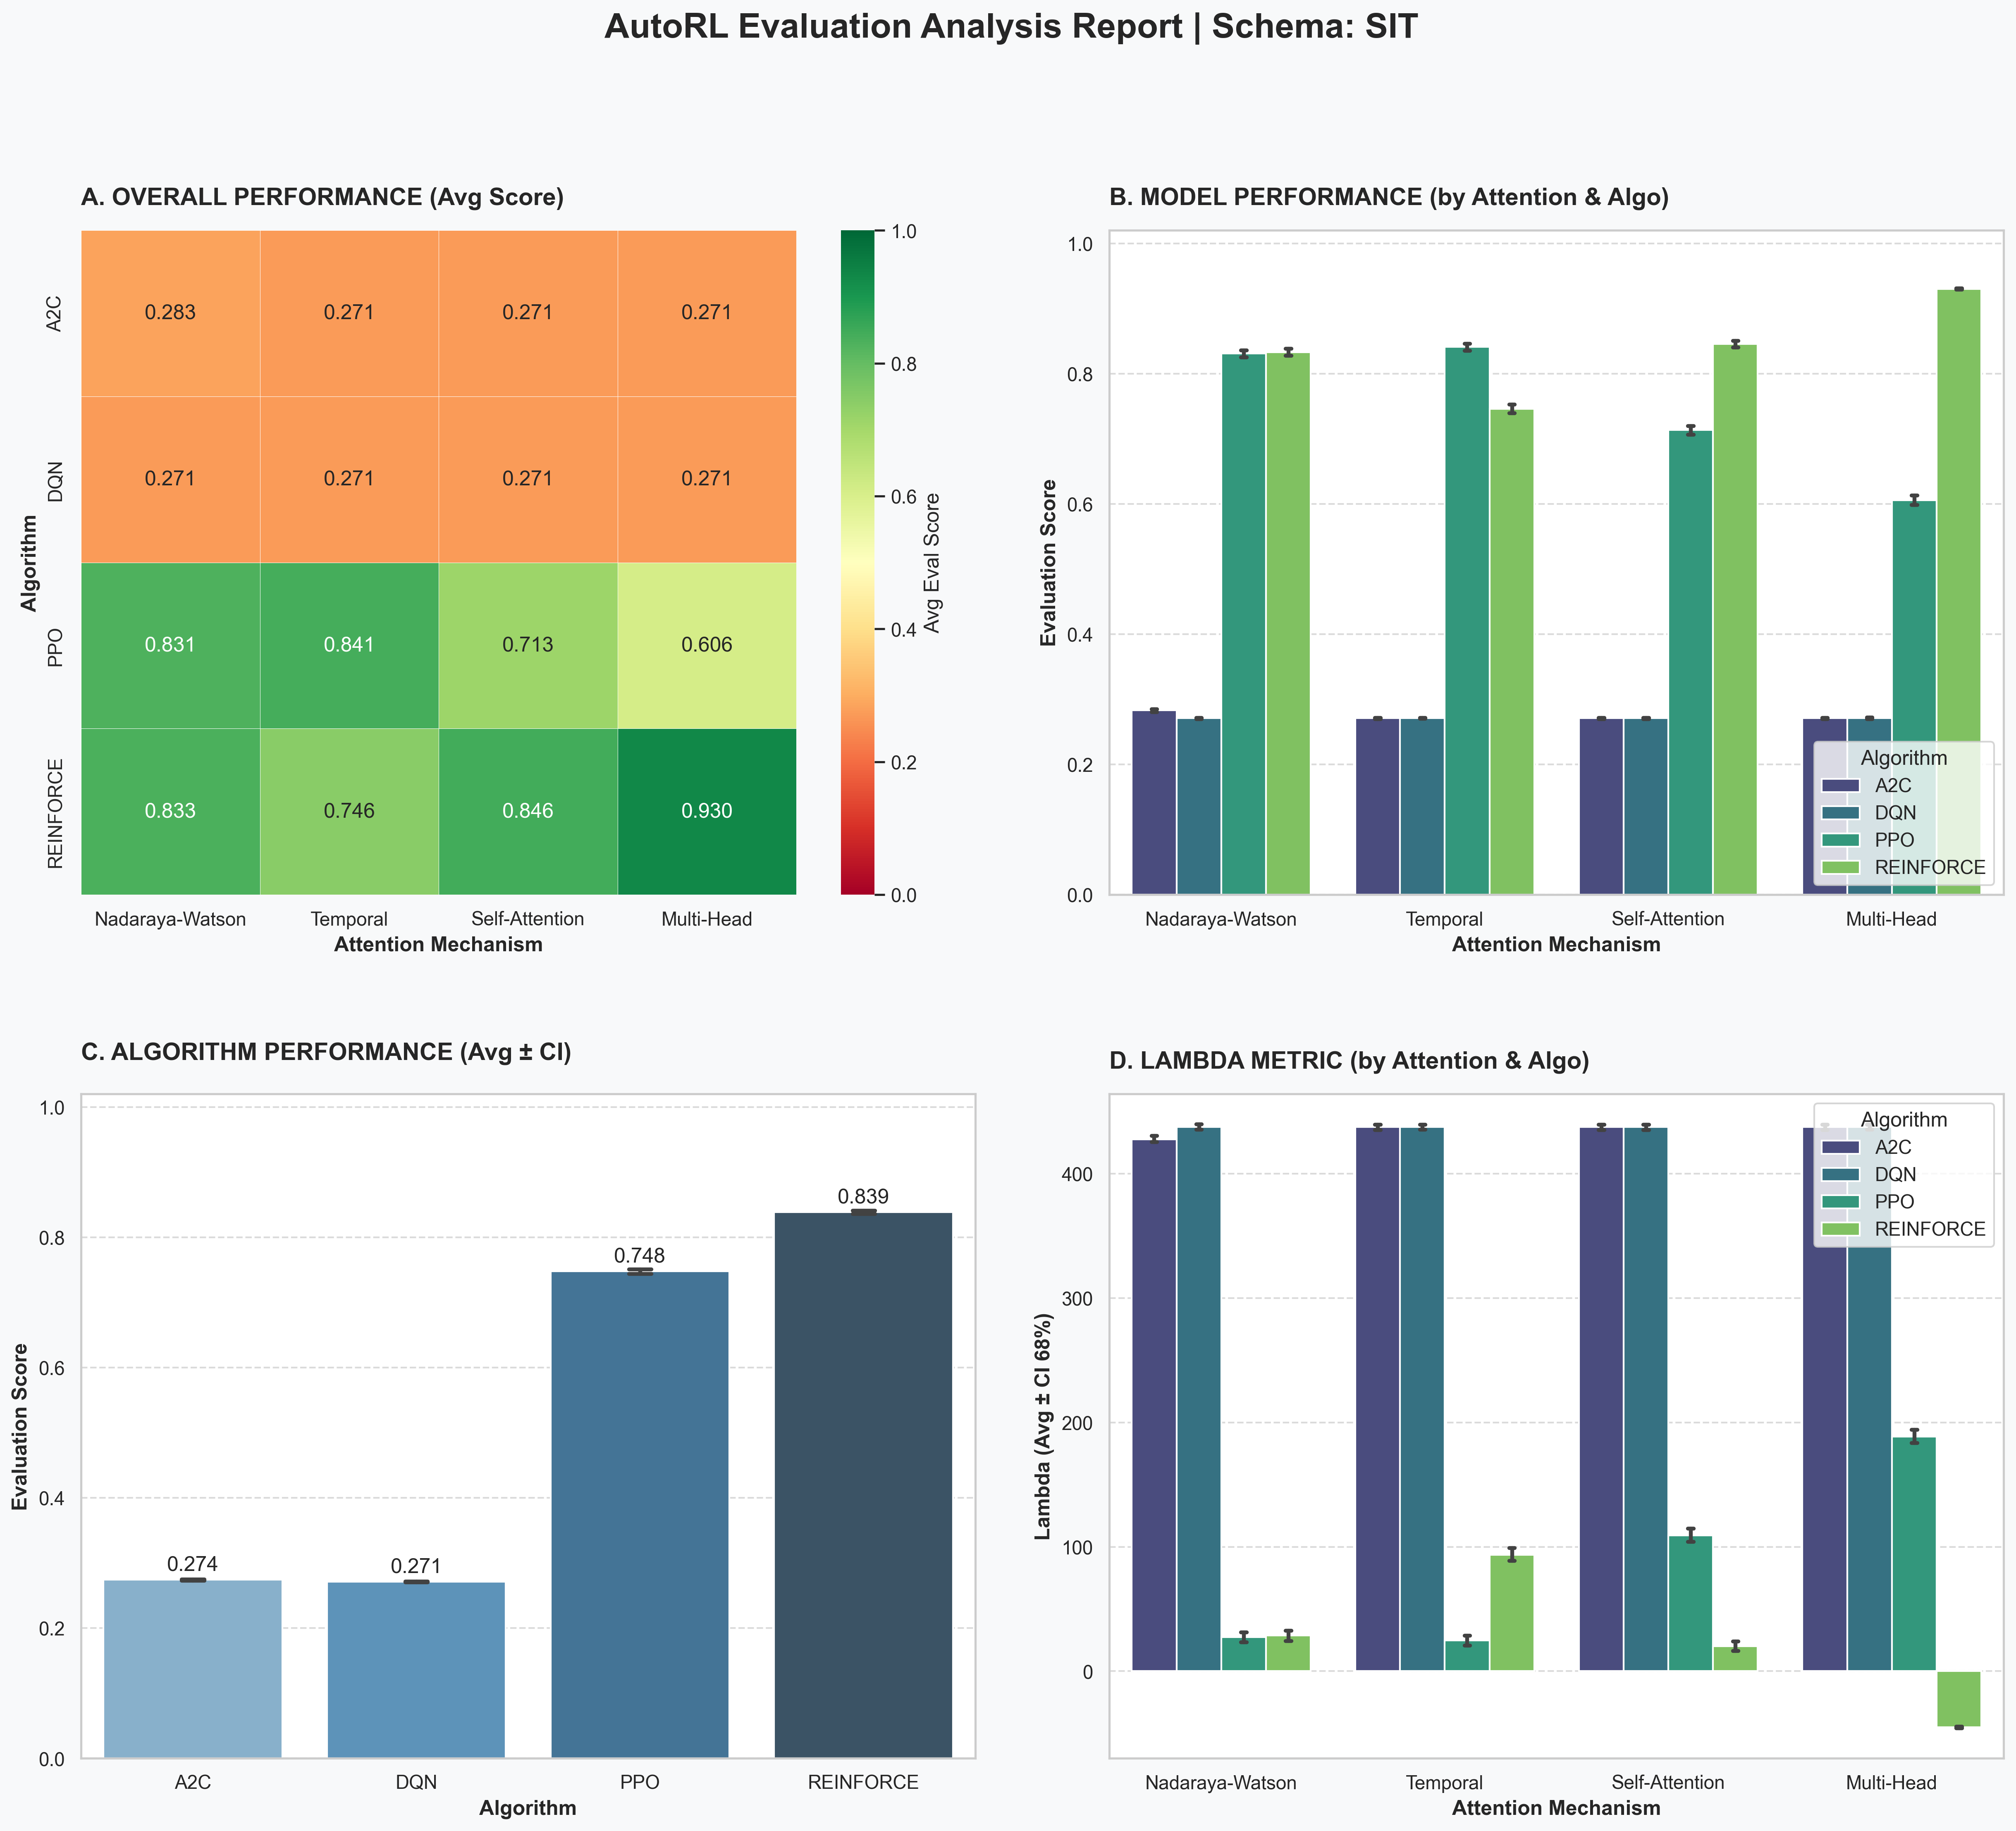
\includegraphics[width=0.95\textwidth]{_Analysis_Report_SIT.png}
        \caption{Consolidated evaluation dashboard for SIT (mean and uncertainty/error bars) used as primary visual evidence for performance patterns across algorithms and attention mechanisms.}
        \label{fig:analysis_sit}
\end{figure}

\begin{figure}[t]
        \centering
        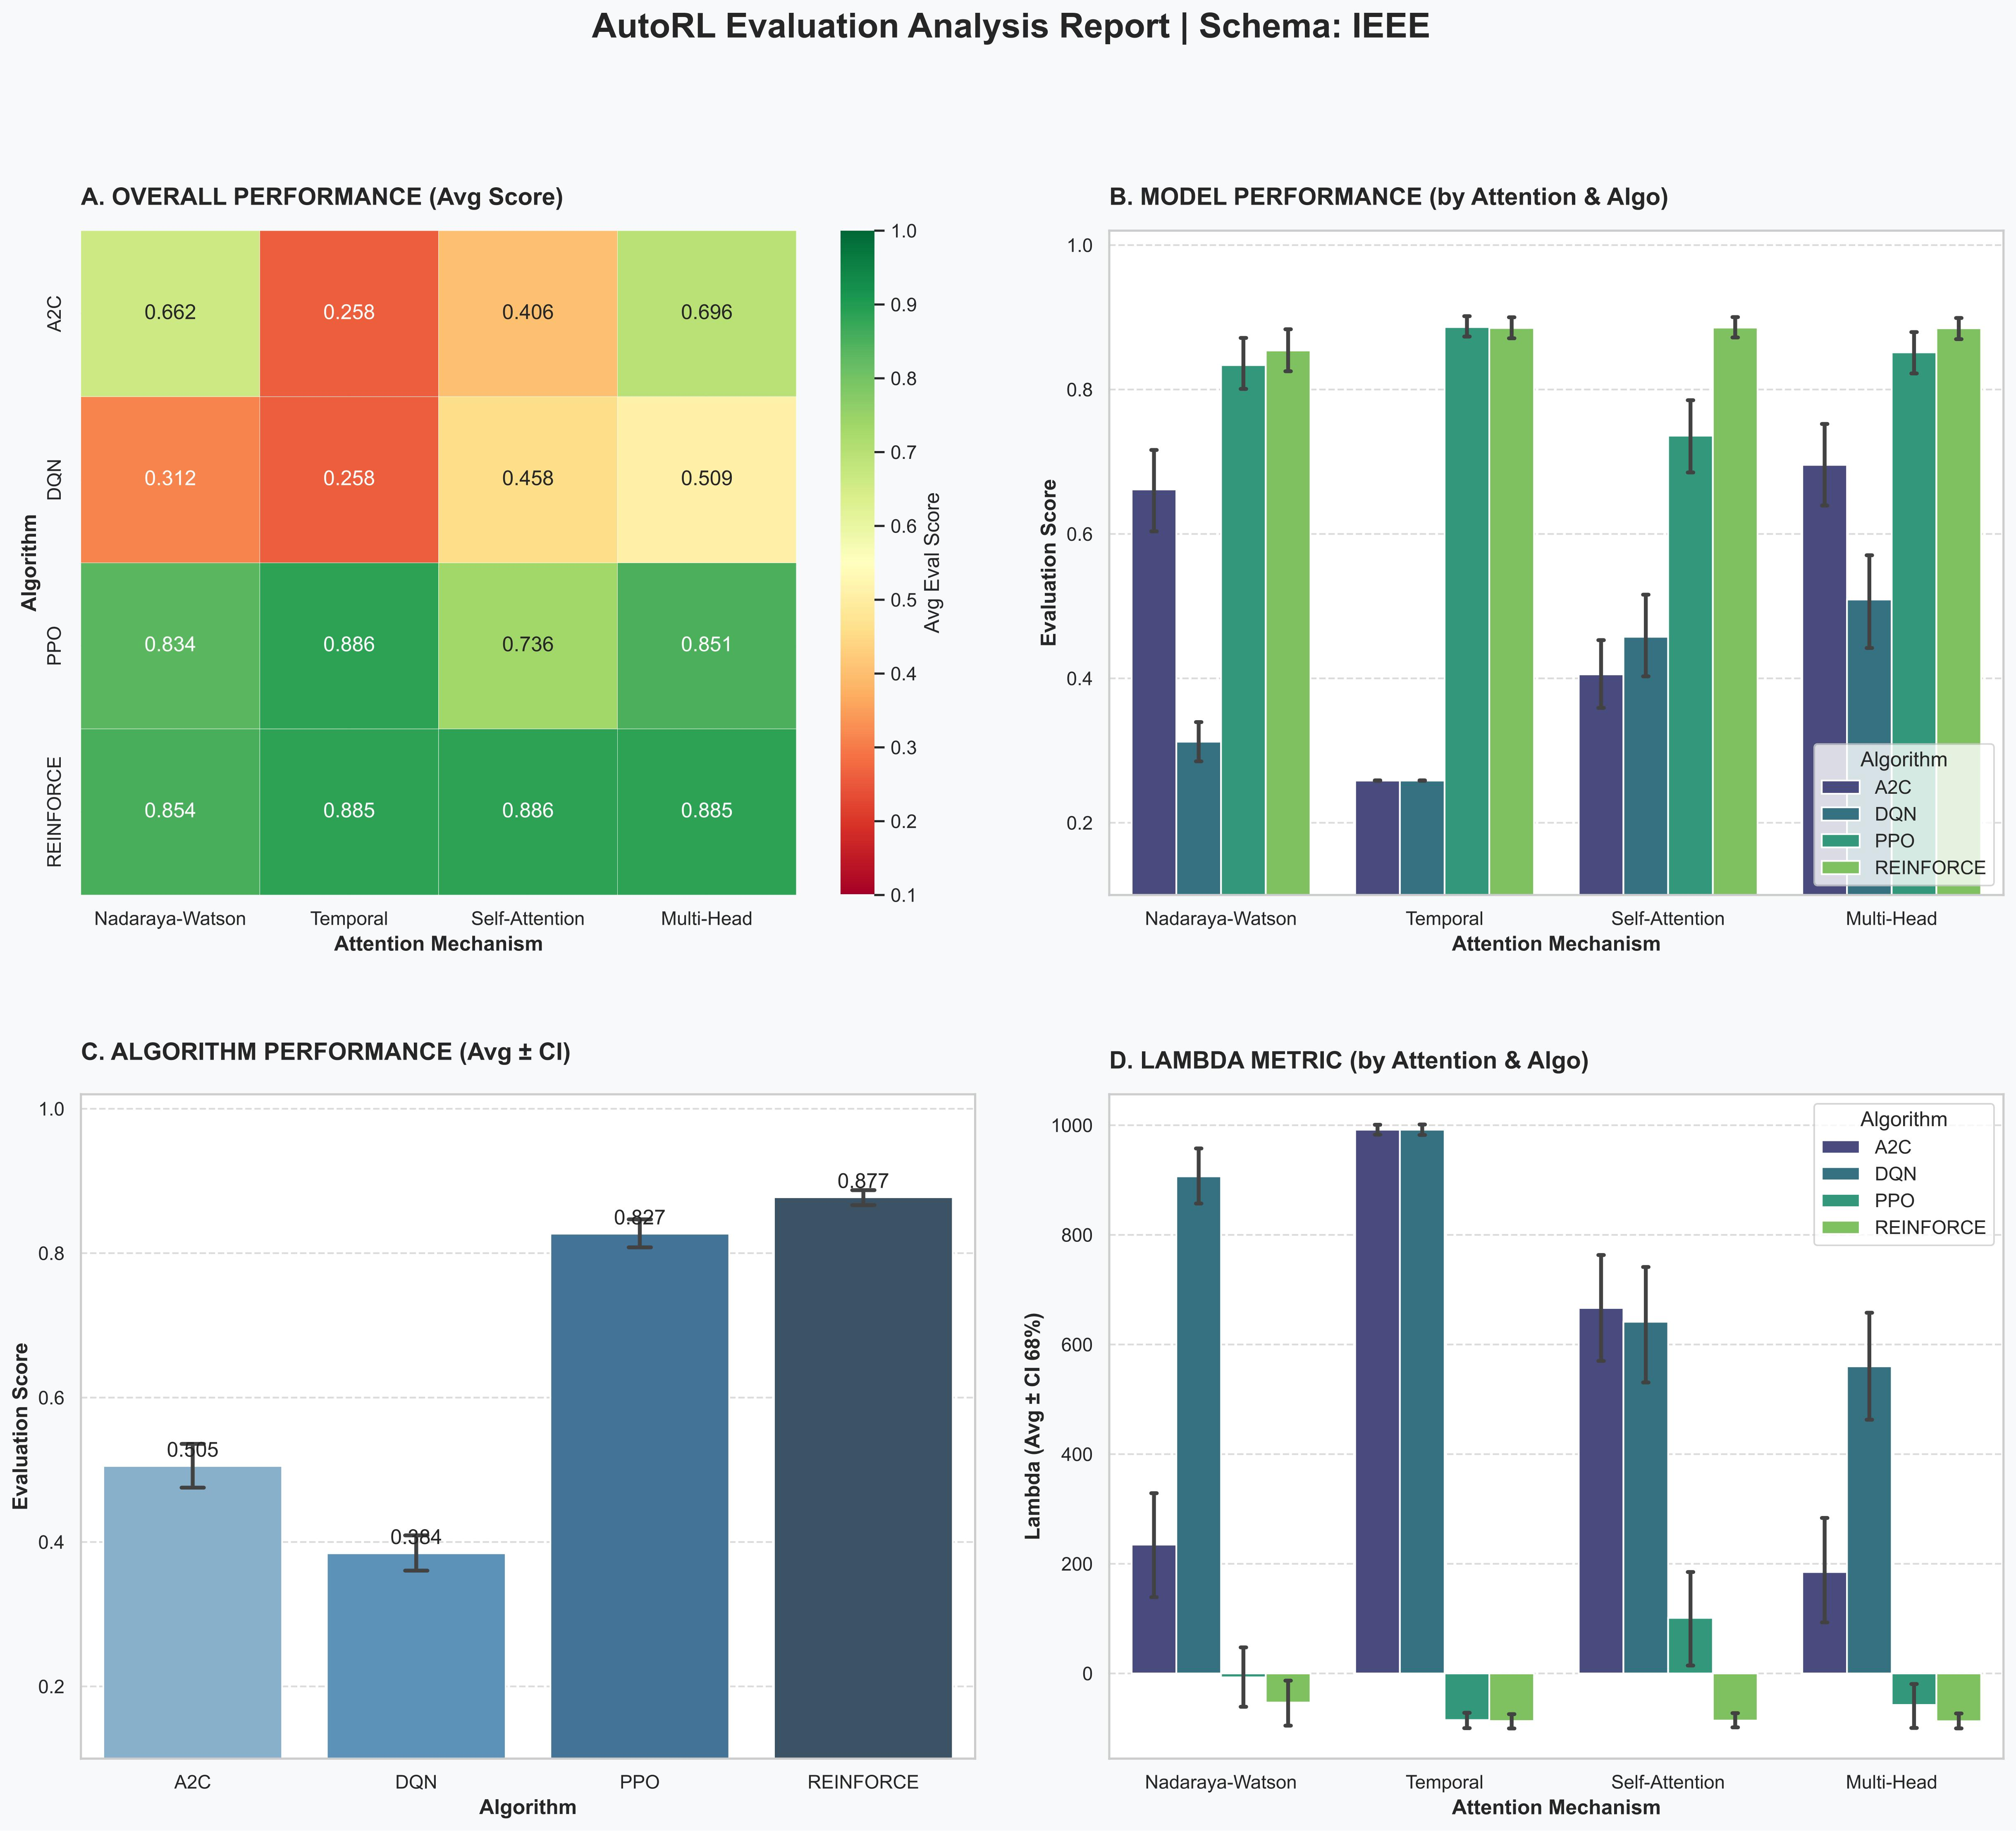
\includegraphics[width=0.95\textwidth]{_Analysis_Report_IEEE.jpg}
        \caption{Consolidated evaluation dashboard for IEEE (mean and uncertainty/error bars) used as primary visual evidence for performance patterns across algorithms and attention mechanisms.}
        \label{fig:analysis_ieee}
\end{figure}

\begin{figure}[t]
        \centering
        \includegraphics[width=0.95\textwidth,height=0.80\textheight,keepaspectratio]{_Heatmap_SIT.png}
        \caption{SIT one-vs-all generalization heatmap: trained models (rows) evaluated on unseen test files (columns).}
        \label{fig:heatmap_sit}
\end{figure}

\begin{figure}[t]
        \centering
        
\includegraphics[width=0.95\textwidth,height=0.80\textheight,keepaspectratio]{_Heatmap_IEEE.jpg}
        \caption{IEEE one-vs-all generalization heatmap: trained models (rows) evaluated on unseen test files (columns).}
        \label{fig:heatmap_ieee}
\end{figure}

\begin{figure}[t]
        \centering
        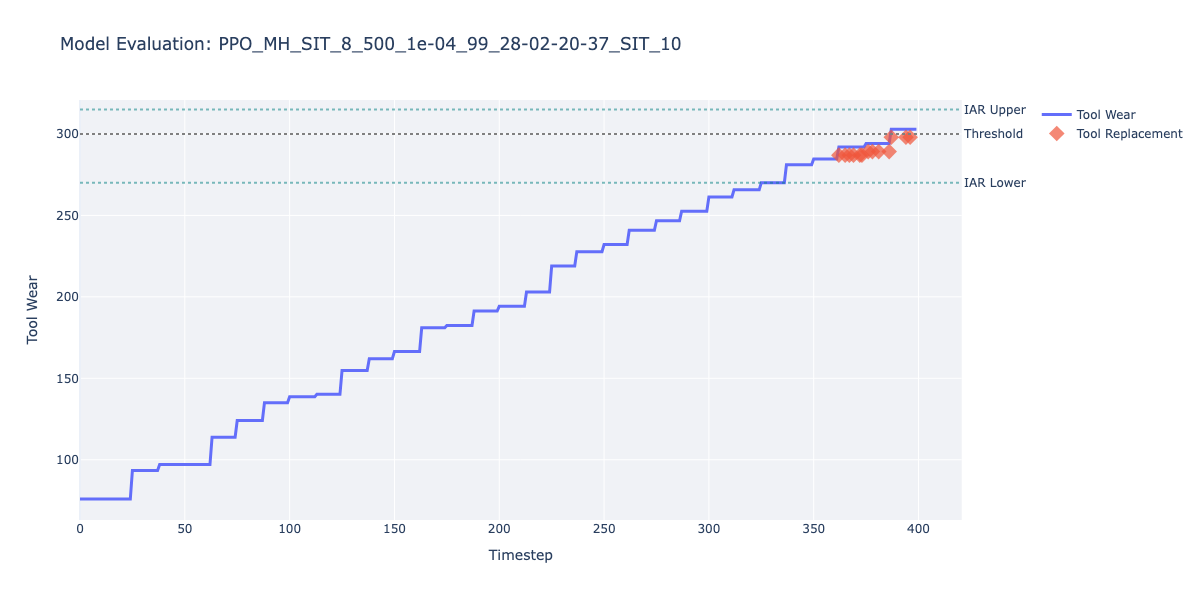
\includegraphics[width=0.48\textwidth]{PPO_MH_SIT_8_10.png}\hfill
        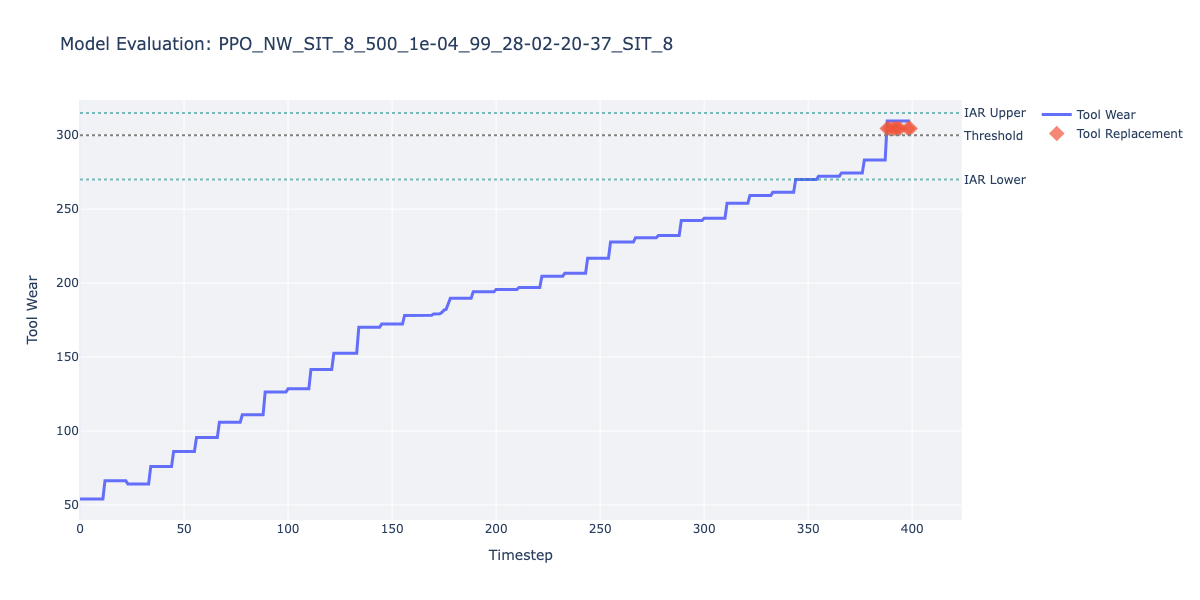
\includegraphics[width=0.48\textwidth]{PPO_NW_SIT_8_10.png}
        \caption{Example unseen-only evaluation traces for PPO on the SIT schema. \textbf{(a)} PPO with Multi-Head attention. \textbf{(b)} PPO with Nadaraya--Watson attention.}
        \label{fig:ppo_unseen_mh_nw}
\end{figure}

%% IEEE REINFORCE + Attention
\begin{figure}[t]
        \centering
        \begin{subfigure}[t]{0.48\textwidth}
                \centering
                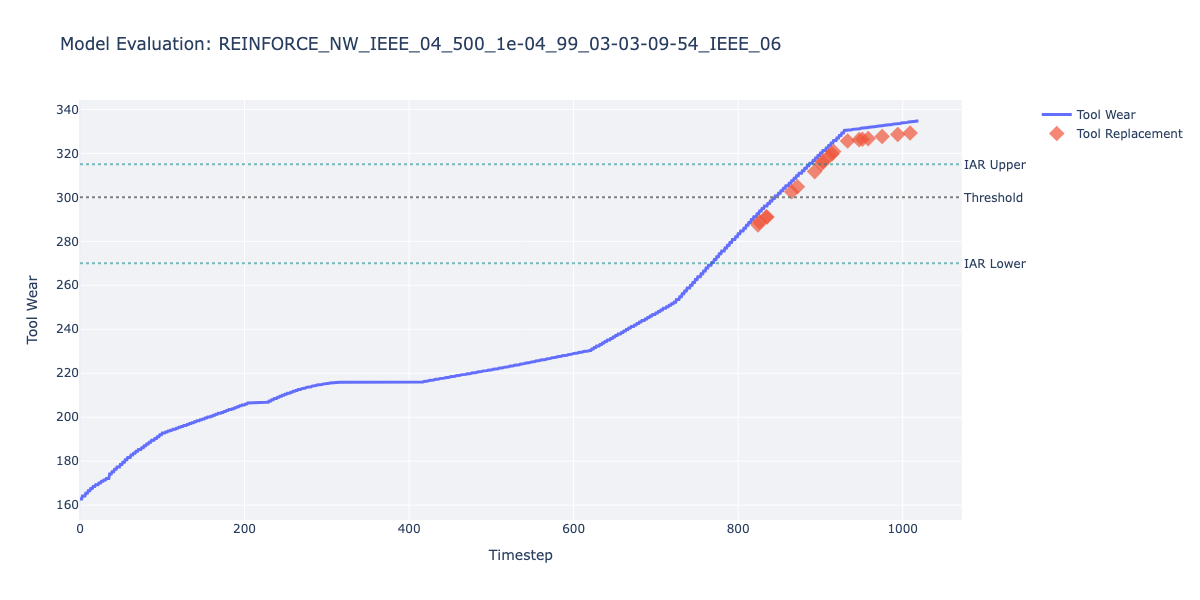
\includegraphics[width=\linewidth]{REINFORCE_NW_IEEE_04_06.png}
                \caption{NW attention}
                \label{fig:IEEE_RF_NW}
        \end{subfigure}\hfill
        \begin{subfigure}[t]{0.48\textwidth}
                \centering
                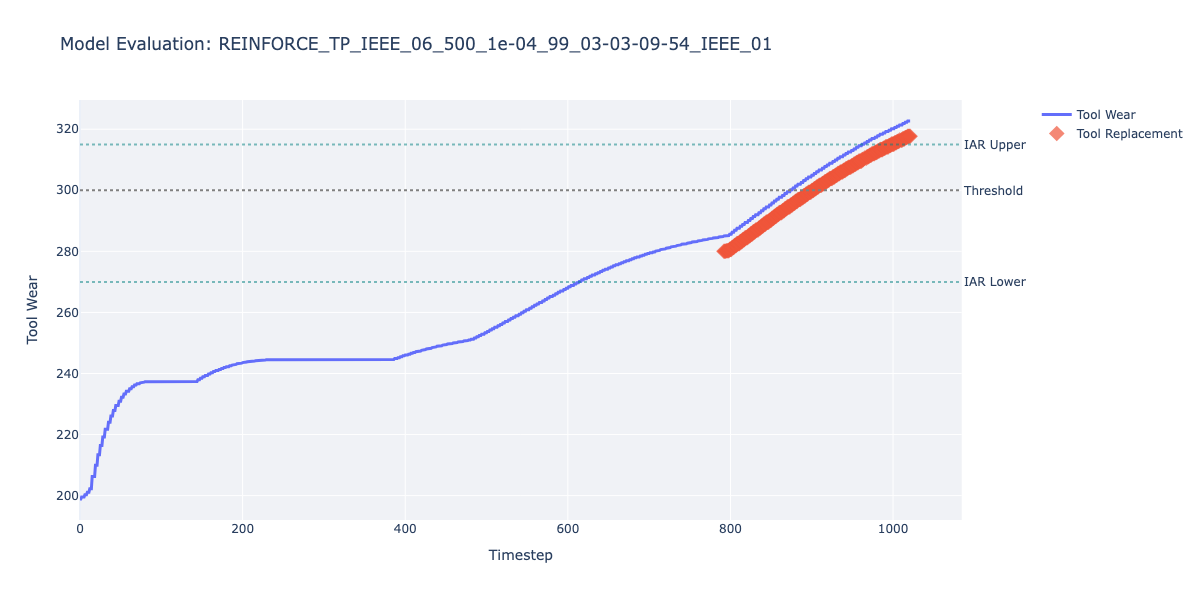
\includegraphics[width=\linewidth]{REINFORCE_TP_IEEE_06_01.png}
                \caption{Temporal attention}
                \label{fig:IEEE_RF_TP}
        \end{subfigure}

        \begin{subfigure}[t]{0.48\textwidth}
                \centering
                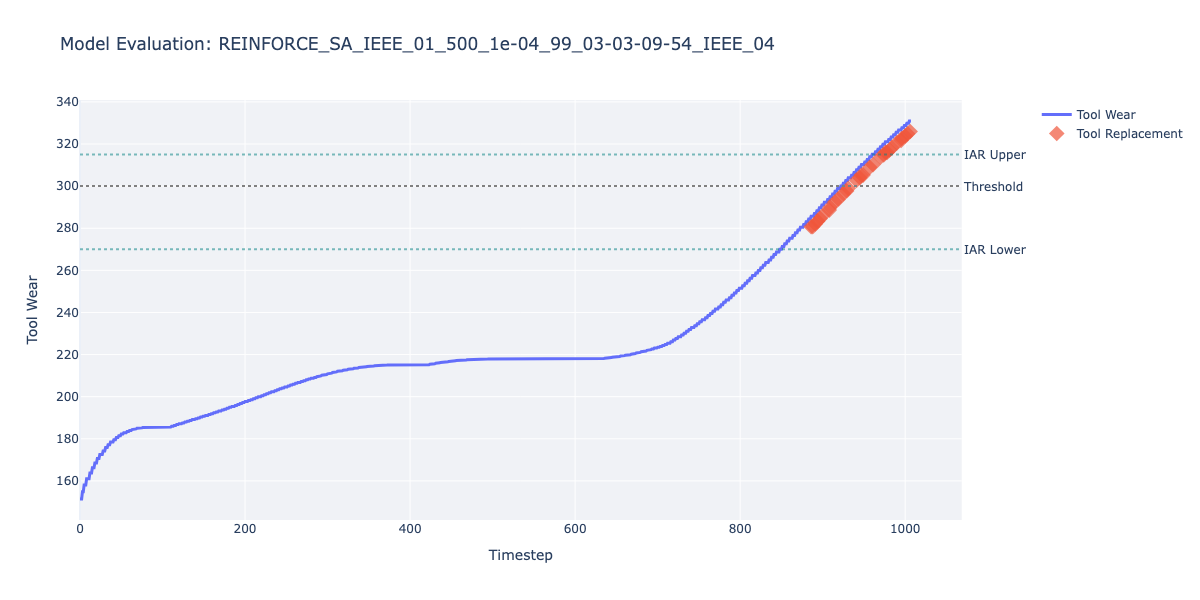
\includegraphics[width=\linewidth]{REINFORCE_SA_IEEE_01_04.png}
                \caption{Self-attention}
                \label{fig:IEEE_RF_SA}
        \end{subfigure}\hfill
        \begin{subfigure}[t]{0.48\textwidth}
                \centering
                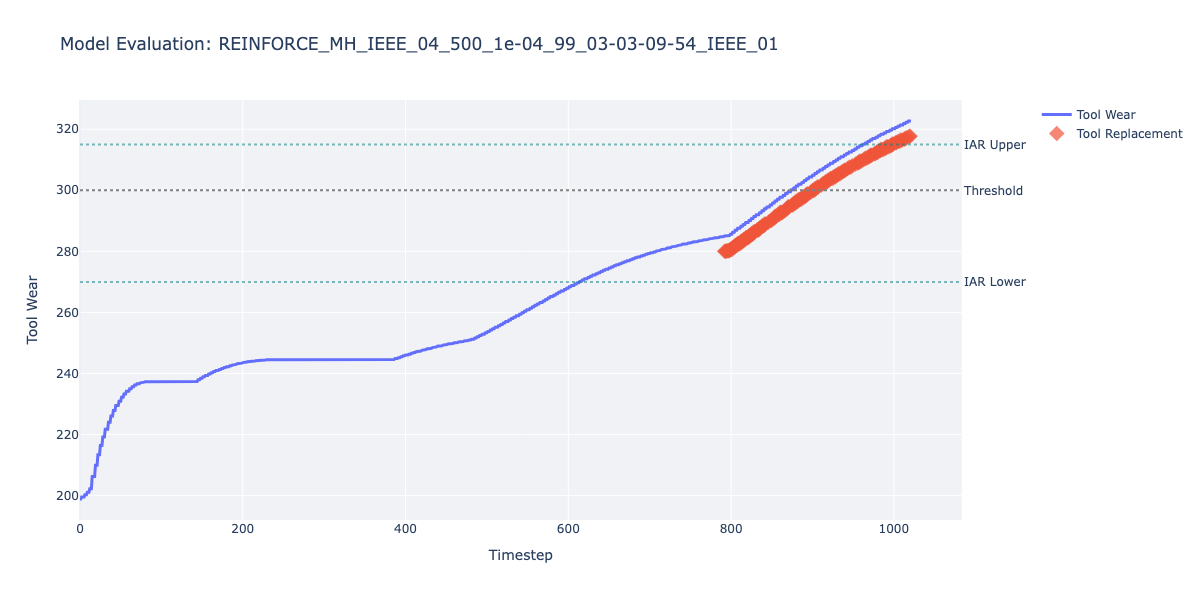
\includegraphics[width=\linewidth]{REINFORCE_MH_IEEE_04_01.png}
                \caption{Multi-head attention}
                \label{fig:IEEE_RF_MH}
        \end{subfigure}

        \caption{Sample evaluation plots showing \textsc{REINFORCE} with different attention mechanisms on the IEEE dataset.}
        \label{fig:IEEE_RF_with_Attention}
\end{figure}

 %% SIT REINFORCE + Attention
\begin{figure}[t]
        \centering
        \begin{subfigure}[t]{0.48\textwidth}
                \centering
                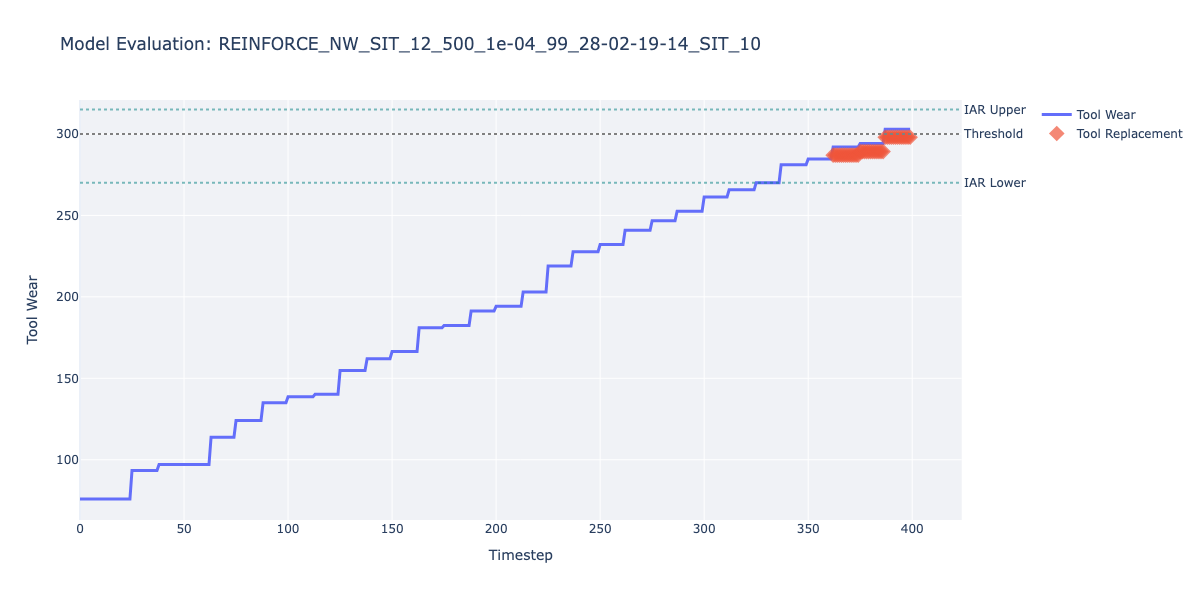
\includegraphics[width=\linewidth]{REINFORCE_NW_SIT_12_10.png}
                \caption{NW attention}
                \label{fig:SIT_RF_NW}
        \end{subfigure}\hfill
        \begin{subfigure}[t]{0.48\textwidth}
                \centering
                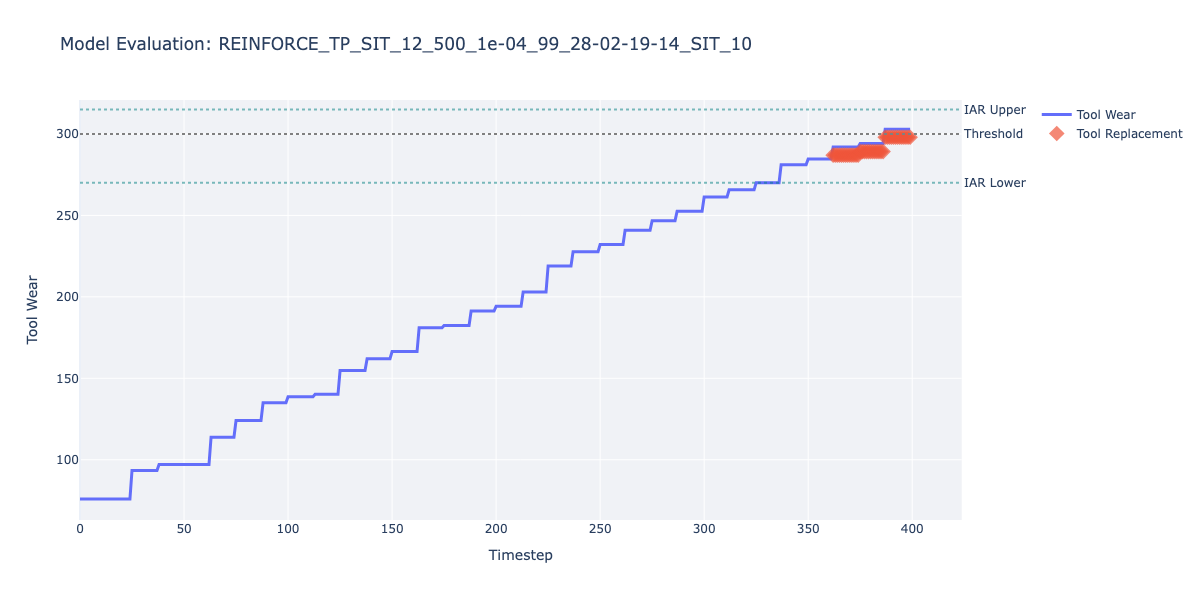
\includegraphics[width=\linewidth]{REINFORCE_TP_SIT_12_10.png}
                \caption{Temporal attention}
                \label{fig:SIT_RF_TP}
        \end{subfigure}

        \begin{subfigure}[t]{0.48\textwidth}
                \centering
                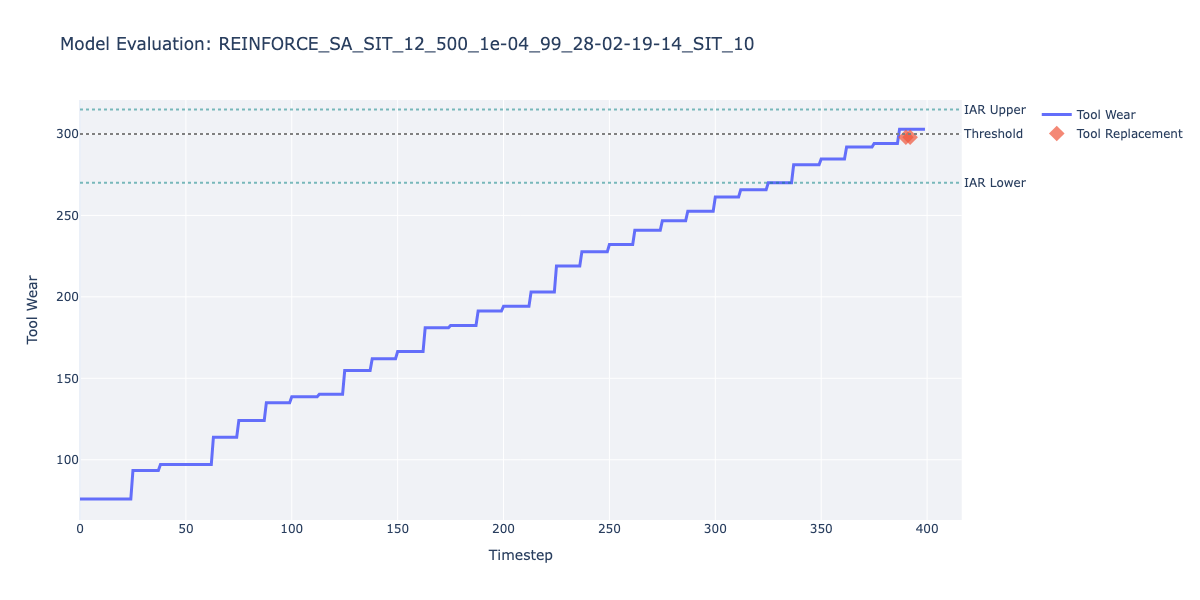
\includegraphics[width=\linewidth]{REINFORCE_SA_SIT_12_10.png}
                \caption{Self-attention}
                \label{fig:SIT_RF_SA}
        \end{subfigure}\hfill
        \begin{subfigure}[t]{0.48\textwidth}
                \centering
                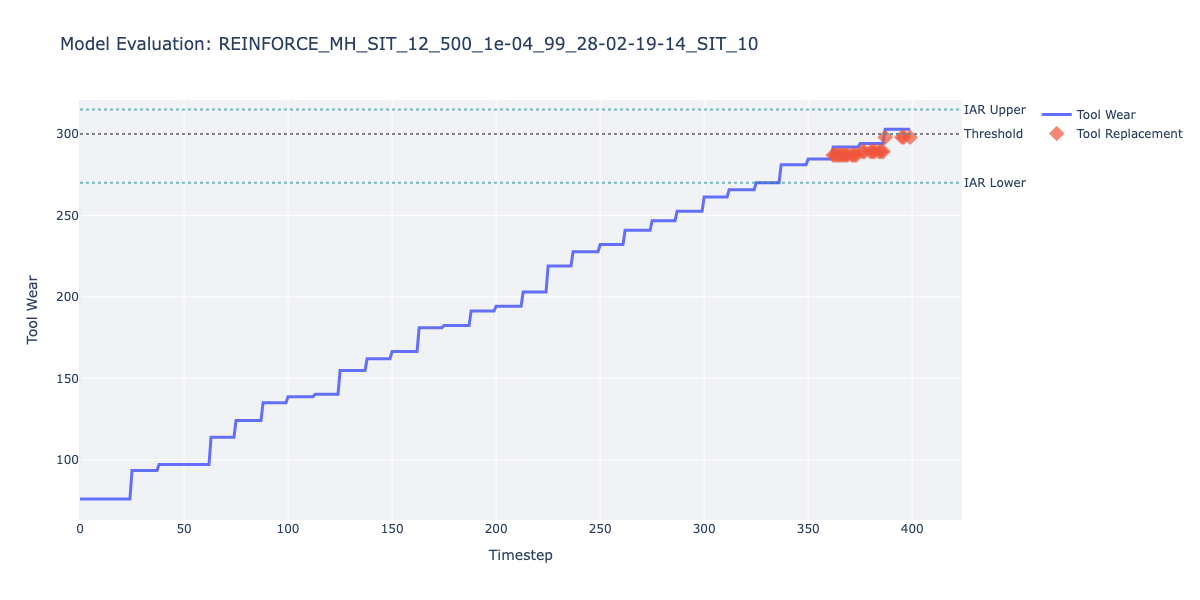
\includegraphics[width=\linewidth]{REINFORCE_MH_SIT_12_10.png}
                \caption{Multi-head attention}
                \label{fig:SIT_RF_MH}
        \end{subfigure}

        \caption{Sample evaluation plots showing \textsc{REINFORCE} with different attention mechanisms on the SIT dataset.}
        \label{fig:SIT_RF_with_Attention}
\end{figure}

\subsection{Pairwise comparison tests: REINFORCE vs A2C/DQN/PPO}
\label{sec:hypothesis_tests}
The hypothesis-test artefacts provide one-tailed Welch $t$-tests at $\alpha=0.05$ for each schema. Table~\ref{tab:hyp_tests} summarizes the unseen-only evaluation-score tests for two reporting panels: \emph{All Attn} and \emph{Best Attn}.

\begin{table}[t]
        \centering
        \caption{Pairwise comparison tests (unseen-only evaluation score): one-tailed Welch $t$-tests comparing REINFORCE to each competitor at $\alpha=0.05$.}
        \label{tab:hyp_tests}
        % (Inlined from figures/hypothesis_tests_summary.tex)
        \begin{tabular}{l l l r r l}
        \toprule
        \textbf{Dataset} & \textbf{Panel} & \textbf{Competitor} & \textbf{t} & \textbf{p (1-tail)} & \textbf{Sig.}\\
        \midrule
        SIT & All Attn & A2C & 198.007 & 0.000 & YES\\
        SIT & Best Attn & A2C & 512.423 & 0.000 & YES\\
        SIT & All Attn & DQN & 202.449 & 0.000 & YES\\
        SIT & Best Attn & DQN & 562.313 & 0.000 & YES\\
        SIT & All Attn & PPO & 20.686 & 0.000 & YES\\
        SIT & Best Attn & PPO & 49.902 & 0.000 & YES\\
        IEEE & All Attn & A2C & 10.726 & 0.000 & YES\\
        IEEE & Best Attn & A2C & 10.434 & 0.000 & YES\\
        IEEE & All Attn & DQN & 15.977 & 0.000 & YES\\
        IEEE & Best Attn & DQN & 15.235 & 0.000 & YES\\
        IEEE & All Attn & PPO & 1.957 & 0.026 & YES\\
        IEEE & Best Attn & PPO & 2.096 & 0.020 & YES\\
        \bottomrule
        \end{tabular}
\end{table}

\subsection{Quantitative IEEE summary (means and 95\% CI)}
\label{sec:ieee_summary}
Table~\ref{tab:ieee_top10} lists the top IEEE configurations by mean evaluation score, and Table~\ref{tab:ieee_best_attn} summarizes the best attention mechanism per algorithm.

\begin{table}[t]
        \centering
        \caption{Top IEEE configurations on unseen-only evaluations (mean and 95\% CI, aggregated across trained models and test files). Numbers are rounded to three decimals.}
        \label{tab:ieee_top10}
        % (Inlined from figures/ieee_unseen_summary.tex)
        \begin{tabular}{ll r r r r}
        \toprule
        \textbf{Algorithm} & \textbf{Attention} & \textbf{Eval. Score} & \textbf{CI} & \textbf{Tool use (\%)} & \textbf{$\lambda$}\\
        \midrule
        PPO & Temporal & 0.886 & 0.031 & 95.199 & -85.050\\
        REINFORCE & Multi-Head & 0.886 & 0.031 & 95.215 & -85.700\\
        REINFORCE & Self-Attention & 0.886 & 0.031 & 95.261 & -86.100\\
        REINFORCE & Temporal & 0.885 & 0.031 & 95.341 & -86.750\\
        PPO & Nadaraya-Watson & 0.857 & 0.070 & 93.651 & -31.900\\
        REINFORCE & Nadaraya-Watson & 0.850 & 0.068 & 93.079 & -40.950\\
        PPO & Multi-Head & 0.843 & 0.070 & 93.170 & -50.300\\
        PPO & Self-Attention & 0.740 & 0.114 & 87.271 & 109.150\\
        A2C & Multi-Head & 0.684 & 0.130 & 82.617 & 208.600\\
        A2C & Nadaraya-Watson & 0.669 & 0.129 & 83.096 & 212.750\\
        \bottomrule
        \end{tabular}
\end{table}

\begin{table}[t]
        \centering
        \caption{IEEE unseen-only: best attention mechanism per algorithm (mean evaluation score and 95\% CI).}
        \label{tab:ieee_best_attn}
        % (Inlined from figures/ieee_best_attention_per_algo.tex)
        \begin{tabular}{l l r r r}
        \toprule
        \textbf{Algorithm} & \textbf{Best attention} & \textbf{Eval. Score} & \textbf{CI} & \textbf{n}\\
        \midrule
        A2C & Multi-Head & 0.684 & 0.130 & 20\\
        DQN & Multi-Head & 0.509 & 0.139 & 20\\
        PPO & Temporal & 0.886 & 0.031 & 20\\
        REINFORCE & Multi-Head & 0.886 & 0.031 & 20\\
        \bottomrule
        \end{tabular}
\end{table}

\subsection{Ablation study / sensitivity analysis: attention mechanisms}
\textbf{Dataset-level interpretation.}
\textbf{SIT (consolidated).} The SIT dashboard (Figure~\ref{fig:analysis_sit}) indicates a clear separation between the two lightweight baselines (A2C/DQN) and the two top performers (PPO/\textsc{REINFORCE}) across attention mechanisms.

\textbf{IEEE.} IEEE results show a tighter competition between PPO and \textsc{REINFORCE}. The best configurations are effectively tied at the reported precision: PPO with temporal attention and \textsc{REINFORCE} with multi-head or self-attention all achieve mean evaluation scores of about 0.886 (Tables~\ref{tab:ieee_top10}--\ref{tab:ieee_best_attn}).

\textbf{Attention effects under H3.}
Attention improves \textsc{REINFORCE}, but no single mechanism dominates across both schemas. On SIT, multi-head attention is the clearest winner and yields the strongest overall \textsc{REINFORCE} configuration. On IEEE, multi-head, self-attention, and temporal attention are all strong, with only marginal differences at the reported precision.

\textbf{Practical recommendation.}
For edge-first deployments with constrained training and inference budgets, \emph{REINFORCE + Multi-Head attention} is a reasonable default for SIT-like settings. For IEEE-like settings, \textsc{REINFORCE}+multi-head, \textsc{REINFORCE}+self-attention, \textsc{REINFORCE}+temporal attention, and PPO+temporal attention appear closely matched.

\subsection{H2: schema portability (SIT vs IEEE)}
H2 is supported structurally by the environment design (Section~\ref{sec:env}) and empirically by results on both schemas (Figures~\ref{fig:analysis_sit}--\ref{fig:heatmap_ieee}). More precisely, the same environment class (with schema detection and feature selection) and the same reward logic (Section~\ref{sec:reward}) can be reused across SIT and IEEE settings while still producing strong policies from online measurements. This is best described as \emph{schema portability} of the environment formulation, not direct train-on-one-schema, test-on-another-schema transfer.
\begin{figure}[t]
        \centering
        \includegraphics[width=0.95\textwidth]{_Statistical_p-value_SIT.png}
        \caption{SIT $p$-value heatmap for hypothesis tests (blue indicates stronger evidence).}
        \label{fig:pvalues_sit}
\end{figure}

\begin{figure}[t]
        \centering
        \includegraphics[width=0.95\textwidth]{_Statistical_p-value_IEEE.jpg}
        \caption{IEEE $p$-value heatmap for hypothesis tests (blue indicates stronger evidence).}
        \label{fig:pvalues_ieee}
\end{figure}

\begin{figure}[t]
        \centering
        \includegraphics[width=0.95\textwidth]{_Statistical_t_SIT.png}
        \caption{SIT $t$-statistic heatmap corresponding to Figure~\ref{fig:pvalues_sit}.}
        \label{fig:tstats_sit}
\end{figure}

\begin{figure}[t]
        \centering
        \includegraphics[width=0.95\textwidth]{_Statistical_t_IEEE.jpg}
        \caption{IEEE $t$-statistic heatmap corresponding to Figure~\ref{fig:pvalues_ieee}.}
        \label{fig:tstats_ieee}
\end{figure}

\subsection{Discussion}
\label{sec:discussion}
\subsubsection{Why lightweight REINFORCE can win in this PdM setup}
The PdM task studied here has a small action space and terminates on replacement, but the policy still has to infer replacement timing from multivariate sensor trajectories rather than from direct inspection measurements. In such settings, representation quality can matter at least as much as optimizer sophistication; this helps explain why a lightweight policy-gradient method paired with suitable feature extraction can compete with heavier baselines.

\subsubsection{Implications for industrial practitioners}
The primary practical implication is that a lightweight policy-gradient learner (\textsc{REINFORCE}), when paired with appropriate attention-based feature extraction, is a viable option for edge-first PdM deployments where model footprint and operational simplicity matter. AutoRL serves as a standardized workflow that automates algorithm and attention sweeps and exposes comparable result artefacts (dashboards, heatmaps, and hypothesis-test summaries) for selection and auditing. A further practical advantage is that the RL agents in this study operate directly on raw sensor observations; by contrast, conventional ML alternatives often require additional feature engineering, target-construction choices, or domain-specific prognostics pipelines.

\subsubsection{Edge compute and sustainability framing}
This paper does not directly measure energy consumption, latency, or deployment memory on target edge hardware. Compute-efficiency is therefore treated here as an engineering motivation, not as a directly validated empirical result. If \textsc{REINFORCE} achieves comparable PdM outcomes to heavier baselines, a simple design principle follows: prefer the least complex method that meets the operational objective \cite{Schwartz2020, Strubell2019}. A subsequent revision will also report direct model-footprint comparisons for the trained policies (e.g., serialized model sizes for PPO versus \textsc{REINFORCE}) to complement the performance analysis.

\section{Conclusion and Future Work}
\label{sec:conclusion}
\subsection{Summary of key findings}
This paper presented an empirical study of \textsc{REINFORCE} with attention mechanisms for milling-machine tool-replacement PdM under edge-oriented constraints. Using a schema-adaptive Gymnasium environment and multi-round evaluation on unseen data, the results indicate a consistent pattern across SIT and IEEE schemas: under the adopted evaluation protocol, \textsc{REINFORCE} emerges as a strong lightweight baseline, performing more strongly than \textsc{A2C} and \textsc{DQN} while remaining comparable to \textsc{PPO}. The study also shows that the same environment formulation and reward logic can be reused effectively across two materially different sensor schemas. Finally, attention is beneficial for \textsc{REINFORCE}, although the most effective choice is schema-dependent: multi-head attention is strongest on SIT, whereas several attention variants perform similarly on IEEE. Interpreted as representation-learning priors, the attention mechanisms bias the policy toward informative sensor patterns in an online monitoring setting.

\subsection{Limitations and threats to validity}
\begin{itemize}
        \item \textbf{Dataset-backed sequential environment:} the environment is sequential and observation-limited, but it is still constructed from logged machining trajectories and models intervention through reward and episode termination rather than through downstream physical process changes; richer closed-loop maintenance dynamics remain for future work.
        \item \textbf{Evaluation dependence:} repeated stochastic evaluation rounds on the same held-out files improve stability estimates but can introduce dependence, so the statistical results should be interpreted alongside the reported mean trends and confidence intervals.
        \item \textbf{Temporal extractor state:} temporal attention maintains an internal timestep counter; production use should ensure the counter resets consistently with episode resets.
        \item \textbf{Missing non-RL baselines:} this study focuses on RL policies that act directly on raw sensor observations. Conventional-ML and prognostics baselines should be included in future comparative studies.
        \item \textbf{Compute and carbon measurement:} energy, latency, memory footprint, and carbon implications are motivated by deployment constraints rather than directly measured on representative edge hardware.
\end{itemize}

\subsection{Future work}
Future work should (i) measure inference latency, serialized model size, and energy on representative edge devices, (ii) incorporate richer maintenance costs and state-estimation models, (iii) add non-RL baselines that operate on the same raw or minimally processed sensor streams, and (iv) evaluate robustness under sensor drift and cross-machine domain shift.



\section*{Acknowledgements}

Acknowledgements are not compulsory. Where included they should be brief. Grant or contribution numbers may be acknowledged.

Please refer to Journal-level guidance for any specific requirements.

\section*{Declarations}

\subsection*{Funding}
The authors received no specific funding for this work.

\subsection*{Conflict of interest/Competing interests}
Not applicable

\subsection*{Ethics approval and consent to participate}
Not applicable

\subsection*{Consent for publication}
Not applicable

\subsection*{Data availability}
The IEEE PHM~2010 milling dataset is publicly available \cite{PHMdata2010}. The SIT dataset used in this study contains in-house experimental measurements and is available from the corresponding author upon reasonable request.

\subsection*{Materials availability}
Not applicable

\subsection*{Code availability}
The code used to train and evaluate the agents (AutoRL pipeline and the Gymnasium environment) is available from the authors upon reasonable request.

\subsection*{Author contribution}
\begin{itemize}
        \item Conceptualization: Rajesh Siraskar, Satish Kumar
        \item Methodology: Rajesh Siraskar, Satish Kumar, Shruti Patil
\end{itemize}

\begin{appendices}

\section{Environment and reward details}
\label{app:env_reward}
\subsection{Observation design rationale}
The environment returns observation vectors comprised only of channels available during cutting. Inspection-based wear measurements are used internally to compute termination and reward.

\subsection{Reward components}
\begin{table}[t]
        \centering
        \caption{Reward shaping components in the milling PdM environment (qualitative summary).}
        \label{tab:reward_components}
        \begin{tabular}{p{0.20\linewidth} p{0.22\linewidth} p{0.50\linewidth}}
                \toprule
                \textbf{Component} & \textbf{Applied when} & \textbf{Effect}\\
                \midrule
                $R_1$ survival reward & continue and safe & Encourages utilization while below threshold.\\
                $R_2$ violation penalty & continue and violate & Strongly discourages threshold violation.\\
                $R_3$ replacement cost & replace action & Regularizes against replacing too early.\\
                $R_4$ near-threshold bonus & replace near $\tau$ & Rewards timely replacement close to threshold.\\
                Stepwise bonuses & wear ratio $\,\ge 0.7, 0.8, 0.9$ & Increases incentive as wear approaches threshold.\\
                \bottomrule
        \end{tabular}
\end{table}

\section{Evaluation protocol details}
\label{app:eval}
\subsection{Multi-round evaluation}
Each agent is evaluated for multiple rounds per test file to reduce variance due to stochastic policies and initialization.

\subsection{Unseen-only emphasis}
This paper focuses on unseen-only evaluation panels for generalization claims (H2). Panels that include self-evaluation are useful for debugging and sanity checks but can overestimate deployment performance.

\section{Dataset schemas and sensor signals}
\label{app:schema}
\begin{table}[t]
\centering
\caption{Sensor channels used as observations by schema (as implemented in \texttt{MT\_Env}).}
\label{tab:schema_features}
\begin{tabular}{p{0.18\linewidth} p{0.75\linewidth}}
\toprule
\textbf{Schema} & \textbf{Observation channels}\\
\midrule
SIT & \texttt{Vib\_Spindle}, \texttt{Vib\_Table}, \texttt{Sound\_Spindle}, \texttt{Sound\_table}, \texttt{X\_Load\_Cell}, \texttt{Y\_Load\_Cell}, \texttt{Z\_Load\_Cell}, \texttt{Current}\\
IEEE & \texttt{force\_x}, \texttt{force\_y}, \texttt{force\_z}, \texttt{vibration\_x}, \texttt{vibration\_y}, \texttt{vibration\_z}, \texttt{acoustic\_emission\_rms}\\
\bottomrule
\end{tabular}
\end{table}

\section{Default constants and hyperparameters}
\label{app:defaults}
\begin{table}[t]
\centering
\caption{Default environment/training constants (from \texttt{code/rl\_pdm.py} and \texttt{code/batch\_train.py}).}
\label{tab:defaults}
\begin{tabular}{p{0.34\linewidth} p{0.18\linewidth} p{0.40\linewidth}}
\toprule
\textbf{Parameter} & \textbf{Default} & \textbf{Meaning}\\
\midrule
\texttt{WEAR\_THRESHOLD} & 300.000 & Wear threshold used for termination and reporting.\\
\texttt{TRAINING\_WEAR\_THRESHOLD} & 300.000 & Training threshold (configurable; default equals threshold).\\
\texttt{EPISODES} & 100 & Training episodes per run (default in RL module).\\
\texttt{LR\_DEFAULT} & 0.001 & Default learning rate (overridden by AutoRL sweep values).\\
\texttt{GAMMA\_DEFAULT} & 0.990 & Default discount factor (overridden by AutoRL sweep values).\\
\texttt{EVAL\_ROUNDS} & 20 & Evaluation rounds per model on unseen data.\\
\texttt{IAR\_RANGE} & 0.050 & IAR bounds range for timing metric computation.\\
\texttt{LAMBDA} & 0.900 & Logistic slack coefficient used in $\lambda$ timing computation.\\
\texttt{R1}, \texttt{R2}, \texttt{R3}, \texttt{R4} & 0.100, -100.000, -0.500, 60.000 & Reward shaping constants.\\
\bottomrule
\end{tabular}
\end{table}

\section{Core code implementation snippets}
\label{app:code_snippets}

\subsection{Nadaraya--Watson attention: forward pass}
\begin{lstlisting}[language=Python,caption={NadarayaWatsonExtractor.forward (code/rl\_pdm.py)},label={lst:nw_forward}]
# NadarayaWatsonExtractor.forward (code/rl_pdm.py)
query = self.query_net(observations)          # q
dist  = (query.unsqueeze(1) - self.keys.unsqueeze(0)).pow(2).sum(dim=2)
beta  = th.exp(self.log_beta)                 # beta > 0
alpha = th.softmax(-beta * dist, dim=1)       # softmax over prototypes
context = (alpha.unsqueeze(2) * self.values.unsqueeze(0)).sum(dim=1)
return context
\end{lstlisting}

\subsection{Temporal attention: forward pass}
\begin{lstlisting}[language=Python,caption={TemporalAttentionExtractor.forward (code/rl\_pdm.py)},label={lst:tp_forward}]
# TemporalAttentionExtractor.forward (code/rl_pdm.py)
spatial_weights = self.spatial_attention(observations)
weighted_spatial = observations * spatial_weights

timestep_idx = int(self.current_timestep.item()) % self.max_timesteps
temporal_encoding = self.positional_encoding[timestep_idx]
temporal_features = temporal_encoding + self.temporal_embedding

combined = th.cat([weighted_spatial, temporal_features.expand(batch_size, -1)], dim=1)
output = self.fusion_net(combined)
self.current_timestep += 1
return output
\end{lstlisting}

\subsection{Multi-head attention: forward pass}
\begin{lstlisting}[language=Python,caption={MultiHeadAttentionExtractor.forward (code/rl\_pdm.py)},label={lst:mh_forward}]
# MultiHeadAttentionExtractor.forward (code/rl_pdm.py)
Q = self.query_proj(observations).view(batch, H, d)
K = self.key_proj(observations).view(batch, H, d)
V = self.value_proj(observations).view(batch, H, d)

scores  = th.einsum('bhd,bhd->bh', Q, K) * self.scale
alpha_h = th.softmax(scores, dim=1).unsqueeze(2)    # softmax over heads
attended = alpha_h * V
concat = attended.view(batch, H * d)
return self.output_proj(concat)
\end{lstlisting}

\subsection{Self-attention: forward pass}
\begin{lstlisting}[language=Python,caption={SelfAttentionExtractor.forward (code/rl\_pdm.py)},label={lst:sa_forward}]
# SelfAttentionExtractor.forward (code/rl_pdm.py)
x = self.input_proj(observations)
Q = self.query(x); K = self.key(x); V = self.value(x)

scores = (Q * K).sum(dim=1, keepdim=True) * self.scale
alpha  = th.softmax(scores, dim=0)          # normalize across batch
attn_output = alpha * V

x = self.norm1(x + attn_output)
x = self.norm2(x + self.ffn(x))
return x
\end{lstlisting}

\subsection{Evaluation score: reference implementation}
\begin{lstlisting}[language=Python,caption={calculate\_eval\_score (code/batch\_train.py)},label={lst:eval_score}]
# calculate_eval_score (code/batch_train.py)
tool_usage_score = min(1.0, max(0.0, tool_usage_pct))
IAR_LOWER = rl_pdm.WEAR_THRESHOLD * (1.0 - rl_pdm.IAR_RANGE)
lambda_score = max(0.0, 1.0 - (abs(lambda_metric) / IAR_LOWER))
violation_score = max(0.0, 1.0 / (1.0 + violations))
eval_score = 0.50*tool_usage_score + 0.30*lambda_score + 0.20*violation_score
\end{lstlisting}

\end{appendices}

\bibliography{JoIM_references}

\end{document}

